\chapter{Wirtinger Flow}

The whole thing about \emph{Wirtinger Flow} variants started with the seminal work of Candes and Soltanolkotabi\cite{wirtinger_flow_cadnes}.
The most important improvements chronologically were done by Candes and Chen\cite{truncated_wirtinger_flow}, Kolte and Özgür\cite{incrementaly_truncated_wirtinger_flow}, and Zhang et al.\cite{reshaped_and_incrementally_reshaped_wirtinger_flow}.
For a quite extensive survey on \emph{Wirtinger Flow} variants please refer to Liu et al.\cite{wirtinger_flow_variants_survey}. Chandra et al.\cite{phase_pack} 
gathered quite number of \emph{Phase Retrieval} methods including a couple of \emph{Wirtinger Flow} variants in the MATLAB\textregistered\space 
problem solving environment in a uniform manner.\\
We quickly go over the problem formulation, difficulties, algorithms, and at the of the chapter we give some numerical experiments we are going
to refer to in the subsequent chapters.

\section{Problem Formulation}
Consider the ray $\boldsymbol{x} \in \mathbb{C}^{n \times 1}$ is emitted onto the object of interest and the diffracted rays are measured as 
$\boldsymbol{y} \in \mathbb{R}^{m \times 1}$ and is connected to the original ray by $\boldsymbol{y} = \varphi(\boldsymbol{A}\boldsymbol{x})$,
where $\boldsymbol{A} \in \mathbb{C}^{m \times n}$ and $\varphi$ the usual element-wise absolute value(or the squared absolute value) from 
$\mathbb{C}^{m \times 1}$ to $\mathbb{R}^{m \times 1}$.\\
Candes and Soltanolkotabi\cite{wirtinger_flow_cadnes} considered $\varphi$ to be squared element-wise absolute value and the loss function to be quadratic. 
The summary for all the variants in terms of formulation is in table\ref{tab:formulation}  


\begin{table}
	\centering
	\begin{tabular}{||c l c||} 
	 \hline
	 \emph{Wirtinger Flow} Variant 			& $\varphi$ 						& loss functions\\ [0.5ex] 
	 \hline\hline
	 Wirtinger Flow 			 			& $\left|\boldsymbol{z}\right|^2$ 	& quadratic 	\\ 
	 Truncated Wirtinger Flow   			& $\left|\boldsymbol{z}\right|^2$ 	& quadratic 	\\
	 Incrementally Truncated Wirtinger Flow & $\left|\boldsymbol{z}\right|^2$  	& quadratic 	\\
	 Reshaped Wirtinger Flow 				& $\left|\boldsymbol{z}\right|$ 	& quadratic 	\\
	 Incrementally Reshaped Flow 			& $\left|\boldsymbol{z}\right|$ 	& quadratic 	\\ [1ex] 
	 \hline
	\end{tabular}
	\caption{$\varphi$ and the loss function used in \cite{wirtinger_flow_cadnes}, \cite{truncated_wirtinger_flow}, \cite{incrementaly_truncated_wirtinger_flow}, \cite{reshaped_and_incrementally_reshaped_wirtinger_flow}}
	\label{tab:formulation}
	\end{table}
\section{Difficulties}

The loss function is non-convex. Set $n=1$, $m=2$, $\boldsymbol{x}_1 = \begin{pmatrix}1+i\end{pmatrix}^{1 \times 1}$, 
$\boldsymbol{x}_2 = \begin{pmatrix}-1-i\end{pmatrix}^{1 \times 1}$, $\boldsymbol{A}=\begin{pmatrix}1\\i \end{pmatrix}^{2 \times 1}$, 
$\boldsymbol{y}=\begin{pmatrix}1\\2 \end{pmatrix}^{2 \times 1}$, and $\lambda=1/2$ to build a counterexample. Non-convexity is bad news for 
optimization as it can be seen vividly in \cite{convex_optimization_boyd} and \cite{numerical_optimization_wright}. To make the matter worse the loss function is not 
holomorphic( it can be easily seen that Cauchy-Riemann equations\cite{papa_rudin} do not hold) and therefore complex differentiability 
is out of the question\cite{papa_rudin}.

% \begin{equation} \label{prob:mainproblem}
% 	Recover $\boldsymbol{x} \in \mathbb{R}^n/\mathbb{C}^n$ from measurements $y_i$ given by
% 	\begin{flalign}
% 		y_i=\left|\langle \boldsymbol{a}_i,\mathbf{x}\rangle\right|, \quad \text{for }\; i=1,\cdots,m, \label{eq:mainproblem}
% 	\end{flalign}
% 	where $\boldsymbol{a}_i \in \mathbb{R}^n/\mathbb{C}^n$ are random design vectors (known). 
% \end{equation}









% \input{./tikz/}
% This file was created with tikzplotlib v0.10.1.
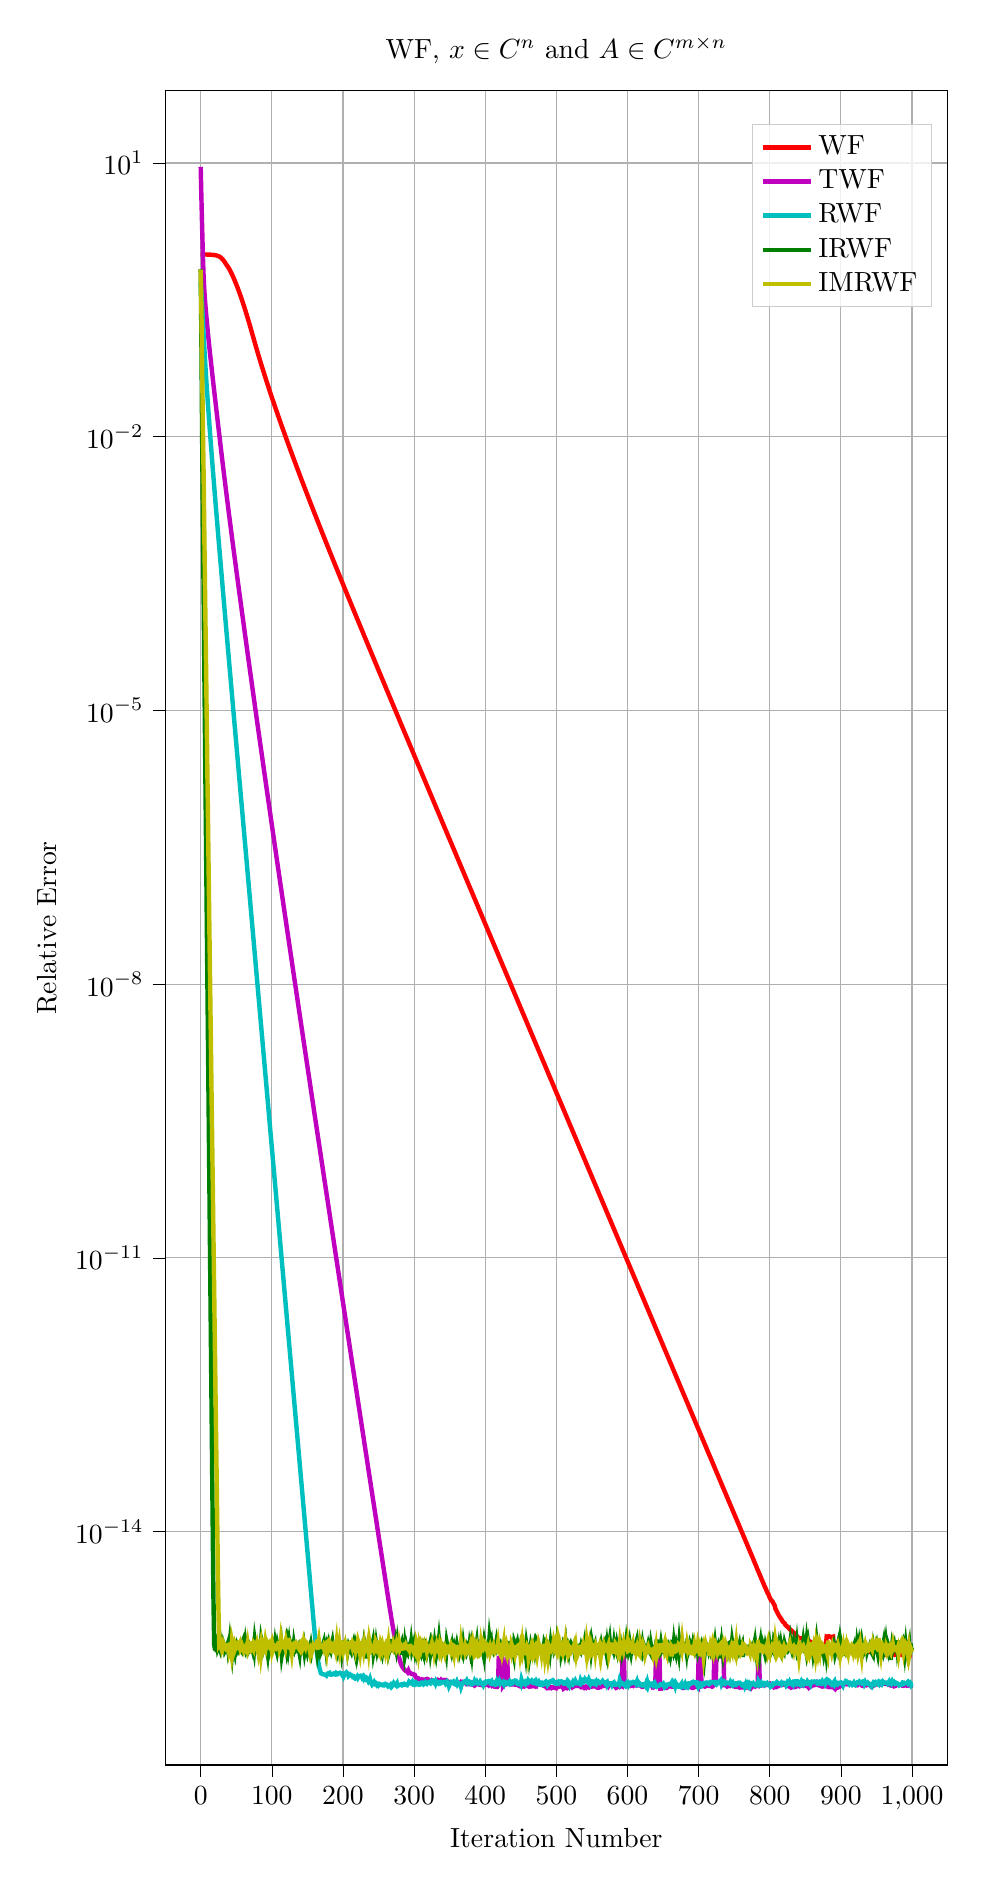
\begin{tikzpicture}

  \definecolor{darkgray176}{RGB}{176,176,176}
  \definecolor{darkturquoise0191191}{RGB}{0,191,191}
  \definecolor{darkviolet1910191}{RGB}{191,0,191}
  \definecolor{goldenrod1911910}{RGB}{191,191,0}
  \definecolor{green01270}{RGB}{0,127,0}
  \definecolor{lightgray204}{RGB}{204,204,204}
  
  \begin{axis}[
  width = 0.95\textwidth,
  height = 65em,
  legend cell align={left},
  legend style={fill opacity=0.8, draw opacity=1, text opacity=1, draw=lightgray204},
  log basis y={10},
  tick align=outside,
  tick pos=left,
  title={\ac{WF}, $\boldsymbol{x} \in \mathbb{C}^n$ and $\boldsymbol{A} \in \mathbb{C}^{m \times n}$},
  x grid style={darkgray176},
  xlabel={Iteration Number},
  xmajorgrids,
  xmin=-50, xmax=1050,
  xtick style={color=black},
  y grid style={darkgray176},
  ylabel={Relative Error},
  ymajorgrids,
  ymin=2.75985430994154e-17, ymax=62.0823981613045,
  ymode=log,
  ytick style={color=black},
  ytick={1e-20,1e-17,1e-14,1e-11,1e-08,1e-05,0.01,10,10000,10000000},
  yticklabels={
    \(\displaystyle {10^{-20}}\),
    \(\displaystyle {10^{-17}}\),
    \(\displaystyle {10^{-14}}\),
    \(\displaystyle {10^{-11}}\),
    \(\displaystyle {10^{-8}}\),
    \(\displaystyle {10^{-5}}\),
    \(\displaystyle {10^{-2}}\),
    \(\displaystyle {10^{1}}\),
    \(\displaystyle {10^{4}}\),
    \(\displaystyle {10^{7}}\)
  }
  ]
  \addplot [ultra thick, red]
  table {%
  0 0.994928926814044
  1 0.994889801322374
  2 0.9948110924516
  3 0.994691466369448
  4 0.994528680803586
  5 0.994319520349983
  6 0.994059697282739
  7 0.993743713960874
  8 0.993364681166018
  9 0.99291408469794
  10 0.99238149021208
  11 0.991754173510616
  12 0.991016660202542
  13 0.990150154746145
  14 0.989131834331593
  15 0.987933977883915
  16 0.986522894863765
  17 0.984857613027563
  18 0.982888279981832
  19 0.980554232400566
  20 0.977781693251186
  21 0.974481078736186
  22 0.970543946166553
  23 0.965839714782401
  24 0.960212483025328
  25 0.953478612680687
  26 0.945426352857586
  27 0.935819773014247
  28 0.924410804833137
  29 0.910965245406331
  30 0.895310514848173
  31 0.877412414927472
  32 0.8574790408091
  33 0.836061583485434
  34 0.814066989041492
  35 0.792548617852663
  36 0.772220197703635
  37 0.752963807003155
  38 0.733884825150826
  39 0.714025149360269
  40 0.693000090215385
  41 0.670983329059018
  42 0.648347450466976
  43 0.625419926827566
  44 0.602424917387903
  45 0.579505372599469
  46 0.556755516118967
  47 0.534244009133946
  48 0.512027351311858
  49 0.490156601962512
  50 0.468680026862704
  51 0.447643427565718
  52 0.427089303002292
  53 0.407055595991651
  54 0.387574510848114
  55 0.368671700155578
  56 0.350365974182052
  57 0.332669564729723
  58 0.315588871540356
  59 0.299125541257913
  60 0.283277687488603
  61 0.268041061017969
  62 0.253410016865008
  63 0.239378186034542
  64 0.225938827429917
  65 0.213084894021537
  66 0.200808886996663
  67 0.189102588781784
  68 0.177956762820528
  69 0.167360890763906
  70 0.157302993482034
  71 0.147769557469904
  72 0.138745567292102
  73 0.130214629950445
  74 0.122194207531744
  75 0.114715875920365
  76 0.107742229478165
  77 0.101237897922956
  78 0.0951695913947969
  79 0.0895061061468954
  80 0.0842182976224538
  81 0.0792790265389404
  82 0.0746630839736293
  83 0.0703471012787694
  84 0.066309450049261
  85 0.0625301365507346
  86 0.0589906941541068
  87 0.0556740765096845
  88 0.0525645534779521
  89 0.0496476112332159
  90 0.0469098574701613
  91 0.0443389322623374
  92 0.0419234248314952
  93 0.0396527962723245
  94 0.0375173081239108
  95 0.0355079565741621
  96 0.0336164120154638
  97 0.0318349636297665
  98 0.0301564686618362
  99 0.0285743060347035
  100 0.0270823339669686
  101 0.0256748512641327
  102 0.0243465619730173
  103 0.0230925431077118
  104 0.0219082151760497
  105 0.0207893152563853
  106 0.0197318723948189
  107 0.018732185112554
  108 0.0177868008315372
  109 0.0168924970437706
  110 0.0160462640656537
  111 0.0152452892334008
  112 0.0144869424090251
  113 0.013768762678642
  114 0.0130884461359962
  115 0.0124438346542306
  116 0.0118329055580804
  117 0.0112537621169671
  118 0.0107046247869587
  119 0.0101838231363354
  120 0.0096897883956122
  121 0.0092210465783894
  122 0.00877621212438497
  123 0.00835398202050114
  124 0.00795313035983832
  125 0.00757250330223691
  126 0.00721101440323959
  127 0.00686764028135981
  128 0.0065414165962461
  129 0.00623143431277761
  130 0.00593683622833792
  131 0.00565681374251461
  132 0.00539060385028484
  133 0.00513748634138757
  134 0.00489678119006975
  135 0.00466784612074251
  136 0.00445007433630639
  137 0.00424289239701482
  138 0.00404575823875369
  139 0.00385815932053163
  140 0.00367961089180879
  141 0.00350965437105164
  142 0.00334785582759109
  143 0.00319380455949235
  144 0.00304711176071818
  145 0.00290740927139265
  146 0.00277434840545062
  147 0.00264759885039635
  148 0.00252684763429543
  149 0.00241179815549035
  150 0.00230216927086696
  151 0.0021976944388062
  152 0.00209812091323959
  153 0.00200320898548528
  154 0.00191273127078192
  155 0.0018264720366558
  156 0.00174422657046002
  157 0.00166580058361045
  158 0.00159100965021516
  159 0.00151967867795246
  160 0.00145164140919975
  161 0.00138673995055006
  162 0.00132482432897895
  163 0.00126575207304
  164 0.00120938781757494
  165 0.00115560293052348
  166 0.00110427516051059
  167 0.00105528830397483
  168 0.0010085318906801
  169 0.000963900886528458
  170 0.000921295412659157
  171 0.000880620479884064
  172 0.00084178573756855
  173 0.000804705236123118
  174 0.000769297202321748
  175 0.000735483826713012
  176 0.000703191062432883
  177 0.000672348434771962
  178 0.00064288886088833
  179 0.000614748479094179
  180 0.000587866487178512
  181 0.000562184989260636
  182 0.000537648850698864
  183 0.000514205560607537
  184 0.000491805101560791
  185 0.000470399826087643
  186 0.000449944339584679
  187 0.000430395389295337
  188 0.00041171175902468
  189 0.000393854169277587
  190 0.000376785182526566
  191 0.000360469113331986
  192 0.000344871943053163
  193 0.000329961238904074
  194 0.000315706077121021
  195 0.000302076970022713
  196 0.000289045796755883
  197 0.000276585737530783
  198 0.000264671211161965
  199 0.000253277815740333
  200 0.000242382272271271
  201 0.000231962371123978
  202 0.000221996921144582
  203 0.000212465701294335
  204 0.000203349414681508
  205 0.000194629644863001
  206 0.000186288814298413
  207 0.000178310144845165
  208 0.000170677620190302
  209 0.000163375950119054
  210 0.000156390536526759
  211 0.000149707441084836
  212 0.000143313354476758
  213 0.00013719556712447
  214 0.000131341941329614
  215 0.000125740884758247
  216 0.000120381325201443
  217 0.000115252686547569
  218 0.000110344865905651
  219 0.000105648211822192
  220 0.000101153503536986
  221 9.68519312263095e-05
  222 9.27350771843695e-05
  223 8.87948978966866e-05
  224 8.50237069614426e-05
  225 8.1414158816783e-05
  226 7.79592332347465e-05
  227 7.46522205440832e-05
  228 7.14867075463782e-05
  229 6.84565640916957e-05
  230 6.55559302814271e-05
  231 6.27792042682607e-05
  232 6.01210306239292e-05
  233 5.75762892476625e-05
  234 5.51400847888807e-05
  235 5.28077365598184e-05
  236 5.05747689140638e-05
  237 4.84369020691682e-05
  238 4.63900433516732e-05
  239 4.44302788447578e-05
  240 4.25538654190495e-05
  241 4.07572231285269e-05
  242 3.90369279542499e-05
  243 3.73897048793828e-05
  244 3.5812421279848e-05
  245 3.43020806158338e-05
  246 3.28558164098592e-05
  247 3.14708864982058e-05
  248 3.01446675425297e-05
  249 2.88746497898422e-05
  250 2.76584320691654e-05
  251 2.64937170136427e-05
  252 2.53783064979009e-05
  253 2.43100972805772e-05
  254 2.32870768424586e-05
  255 2.23073194111884e-05
  256 2.13689821639752e-05
  257 2.04703016001941e-05
  258 1.96095900758276e-05
  259 1.8785232492542e-05
  260 1.79956831342278e-05
  261 1.72394626442257e-05
  262 1.6515155136817e-05
  263 1.58214054369526e-05
  264 1.5156916442257e-05
  265 1.45204466018819e-05
  266 1.39108075066469e-05
  267 1.33268615858532e-05
  268 1.27675199055268e-05
  269 1.22317400636308e-05
  270 1.17185241781542e-05
  271 1.12269169634544e-05
  272 1.07560038910274e-05
  273 1.03049094313477e-05
  274 9.87279537230909e-06
  275 9.45885921150675e-06
  276 9.06233261898803e-06
  277 8.68247996692533e-06
  278 8.31859692353184e-06
  279 7.97000910853766e-06
  280 7.63607080696653e-06
  281 7.31616373904266e-06
  282 7.00969588359499e-06
  283 6.71610035270797e-06
  284 6.43483431493247e-06
  285 6.16537796567527e-06
  286 5.90723354170894e-06
  287 5.65992437881806e-06
  288 5.42299400999908e-06
  289 5.19600530267708e-06
  290 4.97853963328207e-06
  291 4.7701960974222e-06
  292 4.5705907541438e-06
  293 4.37935590282112e-06
  294 4.19613939110675e-06
  295 4.0206039528615e-06
  296 3.85242657435645e-06
  297 3.69129788787673e-06
  298 3.53692159135241e-06
  299 3.38901389292161e-06
  300 3.24730297929986e-06
  301 3.11152850695441e-06
  302 2.9814411151605e-06
  303 2.85680195981666e-06
  304 2.7373822673436e-06
  305 2.62296290752867e-06
  306 2.51333398474704e-06
  307 2.40829444667254e-06
  308 2.30765170956247e-06
  309 2.21122129971287e-06
  310 2.11882651012163e-06
  311 2.03029807182836e-06
  312 1.94547383920507e-06
  313 1.86419848877537e-06
  314 1.78632323079471e-06
  315 1.71170553302934e-06
  316 1.64020885648817e-06
  317 1.57170240218907e-06
  318 1.5060608688799e-06
  319 1.44316422079782e-06
  320 1.38289746568333e-06
  321 1.32515044181081e-06
  322 1.26981761427356e-06
  323 1.21679787998614e-06
  324 1.16599438076968e-06
  325 1.11731432442261e-06
  326 1.07066881348508e-06
  327 1.02597268107283e-06
  328 9.83144333871808e-07
  329 9.42105601568395e-07
  330 9.027815928249e-07
  331 8.65100557242981e-07
  332 8.28993753193294e-07
  333 7.94395321318817e-07
  334 7.61242163180492e-07
  335 7.29473825220449e-07
  336 6.99032387626029e-07
  337 6.6986235775119e-07
  338 6.41910568086543e-07
  339 6.15126078612611e-07
  340 5.8946008323779e-07
  341 5.64865820102195e-07
  342 5.41298485760461e-07
  343 5.18715152985142e-07
  344 4.97074691898391e-07
  345 4.76337694700636e-07
  346 4.56466403178503e-07
  347 4.3742463969459e-07
  348 4.1917774070511e-07
  349 4.01692493364037e-07
  350 3.84937074614267e-07
  351 3.68880992913001e-07
  352 3.53495032451632e-07
  353 3.38751199560624e-07
  354 3.24622671638312e-07
  355 3.11083747906799e-07
  356 2.98109802474763e-07
  357 2.85677239308346e-07
  358 2.7376344907862e-07
  359 2.6234676776523e-07
  360 2.51406437152818e-07
  361 2.40922566800919e-07
  362 2.30876097812313e-07
  363 2.21248767892498e-07
  364 2.12023078071587e-07
  365 2.0318226073883e-07
  366 1.94710249030568e-07
  367 1.86591647438224e-07
  368 1.78811703868386e-07
  369 1.71356282498381e-07
  370 1.64211838167535e-07
  371 1.57365391574898e-07
  372 1.50804505654477e-07
  373 1.44517262854604e-07
  374 1.38492243446779e-07
  375 1.32718504607895e-07
  376 1.27185560662593e-07
  377 1.21883363765551e-07
  378 1.16802285709198e-07
  379 1.11933100351737e-07
  380 1.07266966779569e-07
  381 1.02795413292624e-07
  382 9.85103218269272e-08
  383 9.44039133069121e-08
  384 9.04687334256843e-08
  385 8.66976390421355e-08
  386 8.3083785223591e-08
  387 7.96206127564723e-08
  388 7.630183622648e-08
  389 7.31214325692232e-08
  390 7.00736301159625e-08
  391 6.71528980875188e-08
  392 6.43539365072365e-08
  393 6.16716666290575e-08
  394 5.91012215643061e-08
  395 5.66379376198589e-08
  396 5.42773456736429e-08
  397 5.20151630635331e-08
  398 4.98472858392467e-08
  399 4.77697812872583e-08
  400 4.5778880778578e-08
  401 4.38709729141629e-08
  402 4.20425969557022e-08
  403 4.02904365767587e-08
  404 3.86113137497793e-08
  405 3.70021830622211e-08
  406 3.54601261033224e-08
  407 3.39823462610754e-08
  408 3.2566163516361e-08
  409 3.12090096526895e-08
  410 2.99084236001507e-08
  411 2.86620469339331e-08
  412 2.74676195649695e-08
  413 2.63229756958305e-08
  414 2.52260398356809e-08
  415 2.41748230913395e-08
  416 2.31674194446203e-08
  417 2.22020024628795e-08
  418 2.12768217640645e-08
  419 2.03902000630305e-08
  420 1.95405299602759e-08
  421 1.87262710987751e-08
  422 1.79459473735976e-08
  423 1.71981441851606e-08
  424 1.64815059553257e-08
  425 1.5794733626174e-08
  426 1.51365822950012e-08
  427 1.45058589458179e-08
  428 1.39014203431792e-08
  429 1.33221709090666e-08
  430 1.27670607030322e-08
  431 1.22350836045398e-08
  432 1.17252754428594e-08
  433 1.12367122012092e-08
  434 1.07685083998348e-08
  435 1.03198155096728e-08
  436 9.88982032652754e-09
  437 9.47774357660793e-09
  438 9.08283848389132e-09
  439 8.70438935295511e-09
  440 8.34171036069748e-09
  441 7.99414426544856e-09
  442 7.66106123653392e-09
  443 7.34185765455945e-09
  444 7.03595511700511e-09
  445 6.74279929847523e-09
  446 6.46185898202125e-09
  447 6.19262511139037e-09
  448 5.93460980216855e-09
  449 5.68734557545816e-09
  450 5.45038434530366e-09
  451 5.22329679680135e-09
  452 5.00567146545324e-09
  453 4.79711403378401e-09
  454 4.59724664057701e-09
  455 4.40570712518004e-09
  456 4.22214845753577e-09
  457 4.04623809565342e-09
  458 3.87765728796703e-09
  459 3.71610064579414e-09
  460 3.56127544258686e-09
  461 3.41290118384893e-09
  462 3.27070909946136e-09
  463 3.13444151977912e-09
  464 3.00385157601058e-09
  465 2.8787027322504e-09
  466 2.75876824981638e-09
  467 2.64383083679602e-09
  468 2.53368228189796e-09
  469 2.42812304110307e-09
  470 2.32696188038652e-09
  471 2.23001555088027e-09
  472 2.13710842868059e-09
  473 2.04807218589028e-09
  474 1.96274559178198e-09
  475 1.88097400911874e-09
  476 1.80260935254012e-09
  477 1.72750967564285e-09
  478 1.65553890209505e-09
  479 1.58656667217044e-09
  480 1.52046806181917e-09
  481 1.45712332843054e-09
  482 1.39641775225556e-09
  483 1.33824132485521e-09
  484 1.28248869917167e-09
  485 1.22905891706233e-09
  486 1.17785510915889e-09
  487 1.12878462183718e-09
  488 1.08175851408939e-09
  489 1.03669163970082e-09
  490 9.93502329613949e-10
  491 9.52112413498841e-10
  492 9.12446882425152e-10
  493 8.74433877683738e-10
  494 8.38004582294118e-10
  495 8.030929926375e-10
  496 7.69635869858859e-10
  497 7.3757263613326e-10
  498 7.06845208691388e-10
  499 6.77397934146045e-10
  500 6.49177463899373e-10
  501 6.22132699550229e-10
  502 5.9621466107916e-10
  503 5.71376397447256e-10
  504 5.47572929841319e-10
  505 5.24761121305615e-10
  506 5.02899683128275e-10
  507 4.81949022283303e-10
  508 4.61871180629534e-10
  509 4.42629778439634e-10
  510 4.24189996096677e-10
  511 4.06518428321709e-10
  512 3.89583073644612e-10
  513 3.73353241273725e-10
  514 3.57799554201385e-10
  515 3.42893841806377e-10
  516 3.28609124619085e-10
  517 3.14919492036584e-10
  518 3.01800172904122e-10
  519 2.89227415017814e-10
  520 2.7717841502729e-10
  521 2.65631402057773e-10
  522 2.54565426520125e-10
  523 2.43960471642517e-10
  524 2.33797309765857e-10
  525 2.24057538175596e-10
  526 2.14723534385123e-10
  527 2.05778387857536e-10
  528 1.972058775903e-10
  529 1.88990501061444e-10
  530 1.81117379586164e-10
  531 1.73572253633524e-10
  532 1.66341434557314e-10
  533 1.59411869874092e-10
  534 1.52770971977105e-10
  535 1.46406730129147e-10
  536 1.40307611962458e-10
  537 1.34462592379144e-10
  538 1.28861070055067e-10
  539 1.23492892810764e-10
  540 1.18348346833652e-10
  541 1.13418129931075e-10
  542 1.08693303987551e-10
  543 1.04165301666659e-10
  544 9.98259437886797e-11
  545 9.56673575223395e-11
  546 9.16820066996765e-11
  547 8.78626771524395e-11
  548 8.42024683914781e-11
  549 8.06947174361451e-11
  550 7.73331174343343e-11
  551 7.41115393397883e-11
  552 7.10241801101722e-11
  553 6.80654231180942e-11
  554 6.5229934563085e-11
  555 6.25125798602891e-11
  556 5.99084172151819e-11
  557 5.74127453753494e-11
  558 5.50210290435903e-11
  559 5.27289460216408e-11
  560 5.05323587077791e-11
  561 4.84272831789177e-11
  562 4.64099037405262e-11
  563 4.44765462155274e-11
  564 4.26237249038573e-11
  565 4.08481200733411e-11
  566 3.91464647269056e-11
  567 3.75156945615699e-11
  568 3.59528656097917e-11
  569 3.4455140480601e-11
  570 3.30198025112015e-11
  571 3.16442568842366e-11
  572 3.0326029559279e-11
  573 2.90626948985221e-11
  574 2.78520150750585e-11
  575 2.66917601371049e-11
  576 2.55798394005698e-11
  577 2.451421733701e-11
  578 2.3493015410012e-11
  579 2.25143398724965e-11
  580 2.15764561683243e-11
  581 2.06776104614038e-11
  582 1.98162284157176e-11
  583 1.89907218377156e-11
  584 1.81996151616836e-11
  585 1.74414531156668e-11
  586 1.67148871473909e-11
  587 1.60185756578585e-11
  588 1.53512845199536e-11
  589 1.47117750869691e-11
  590 1.40988946637448e-11
  591 1.35115807442873e-11
  592 1.29487003440871e-11
  593 1.2409297690112e-11
  594 1.18923395680975e-11
  595 1.13969344489616e-11
  596 1.09221681215638e-11
  597 1.04671777158867e-11
  598 1.00311432946221e-11
  599 9.61325995083323e-12
  600 9.21279439610189e-12
  601 8.82900402479421e-12
  602 8.46119852552288e-12
  603 8.1087311109816e-12
  604 7.77094166792565e-12
  605 7.44721751706618e-12
  606 7.13698252200446e-12
  607 6.83967518353553e-12
  608 6.55474140520384e-12
  609 6.28168980301095e-12
  610 6.01999995016768e-12
  611 5.76922211258653e-12
  612 5.52889739292748e-12
  613 5.29856807119053e-12
  614 5.07784460238819e-12
  615 4.86630863043291e-12
  616 4.66359585105998e-12
  617 4.46932726989057e-12
  618 4.28314501603398e-12
  619 4.1047384587479e-12
  620 3.9337360991479e-12
  621 3.7698541972069e-12
  622 3.61281403765992e-12
  623 3.46229914012286e-12
  624 3.31808391113964e-12
  625 3.17984748236729e-12
  626 3.04739047399313e-12
  627 2.92044463097857e-12
  628 2.79879082332974e-12
  629 2.6821920942687e-12
  630 2.57043474903452e-12
  631 2.46335541998292e-12
  632 2.36073894319659e-12
  633 2.2624041186992e-12
  634 2.16816797385201e-12
  635 2.07783724325157e-12
  636 1.99127529407544e-12
  637 1.90831200507567e-12
  638 1.82881810816075e-12
  639 1.75262313792846e-12
  640 1.67962134925889e-12
  641 1.60964728561233e-12
  642 1.5426045482627e-12
  643 1.47834951176366e-12
  644 1.41675348773345e-12
  645 1.3577418247726e-12
  646 1.30118477581877e-12
  647 1.2469796261512e-12
  648 1.19504156758345e-12
  649 1.14525591271469e-12
  650 1.09755217088239e-12
  651 1.05180148405235e-12
  652 1.00799069642174e-12
  653 9.66000394948316e-13
  654 9.25752570731579e-13
  655 8.87203723857278e-13
  656 8.50237018671334e-13
  657 8.14804747681908e-13
  658 7.80882581093107e-13
  659 7.48334780523031e-13
  660 7.17168166321027e-13
  661 6.87297651680458e-13
  662 6.58675651821384e-13
  663 6.31240508233869e-13
  664 6.04948308234992e-13
  665 5.7973971912222e-13
  666 5.55580942037984e-13
  667 5.32439500903947e-13
  668 5.10261988891375e-13
  669 4.89018586950854e-13
  670 4.68621447968574e-13
  671 4.49116269443834e-13
  672 4.30409029849186e-13
  673 4.12469855529496e-13
  674 3.95267950316317e-13
  675 3.78809188714553e-13
  676 3.63028073782438e-13
  677 3.47904544922094e-13
  678 3.33407152817179e-13
  679 3.19519735057983e-13
  680 3.06196360959863e-13
  681 2.93441803176494e-13
  682 2.81221757572548e-13
  683 2.69513194454155e-13
  684 2.58281831728903e-13
  685 2.47524684319599e-13
  686 2.37212470597229e-13
  687 2.27321546115564e-13
  688 2.17856748886206e-13
  689 2.08785819044224e-13
  690 2.00081795850845e-13
  691 1.91739702149109e-13
  692 1.83759822647381e-13
  693 1.76113712609602e-13
  694 1.68764080162326e-13
  695 1.61742310999548e-13
  696 1.5500305981756e-13
  697 1.48543076468571e-13
  698 1.42355471405409e-13
  699 1.36427120924725e-13
  700 1.3073184010248e-13
  701 1.25284691288701e-13
  702 1.20074488295847e-13
  703 1.15082717472651e-13
  704 1.10284567389878e-13
  705 1.05697331871536e-13
  706 1.01291969183321e-13
  707 9.70708183951969e-14
  708 9.30217796278084e-14
  709 8.91512421647708e-14
  710 8.54358158960462e-14
  711 8.187295772643e-14
  712 7.8458538530681e-14
  713 7.51827792994565e-14
  714 7.20346025530763e-14
  715 6.90476995624045e-14
  716 6.61749321178506e-14
  717 6.342303637818e-14
  718 6.07894801238543e-14
  719 5.82418358917794e-14
  720 5.58141171650849e-14
  721 5.34849845833849e-14
  722 5.12462641396775e-14
  723 4.91167713981155e-14
  724 4.70678788230413e-14
  725 4.51069445247908e-14
  726 4.32368577682439e-14
  727 4.14273059005149e-14
  728 3.96907416773793e-14
  729 3.80514514860661e-14
  730 3.64724944516589e-14
  731 3.49456714825651e-14
  732 3.34747809441484e-14
  733 3.20838629609485e-14
  734 3.07446303043473e-14
  735 2.94659975483542e-14
  736 2.82455167846212e-14
  737 2.70802597376117e-14
  738 2.59429295089336e-14
  739 2.48619419803728e-14
  740 2.38246107058405e-14
  741 2.28387032434969e-14
  742 2.18769193587138e-14
  743 2.09797331950782e-14
  744 2.01175998045365e-14
  745 1.92651484338402e-14
  746 1.84792815872123e-14
  747 1.7703876394623e-14
  748 1.69592644839404e-14
  749 1.6261663055569e-14
  750 1.55921533672966e-14
  751 1.49439722801353e-14
  752 1.43252884516428e-14
  753 1.37285237920604e-14
  754 1.31546658230721e-14
  755 1.26150210473481e-14
  756 1.20863342502337e-14
  757 1.15845021252601e-14
  758 1.10829441285404e-14
  759 1.06251180467931e-14
  760 1.01911594828729e-14
  761 9.75303519338794e-15
  762 9.37601268991388e-15
  763 8.96190652502935e-15
  764 8.60267858390589e-15
  765 8.23118898773918e-15
  766 7.89047518068416e-15
  767 7.57032499334589e-15
  768 7.26251543474986e-15
  769 6.94813856203655e-15
  770 6.6582520746129e-15
  771 6.37530780488878e-15
  772 6.1133993830077e-15
  773 5.85361469343813e-15
  774 5.61963948134739e-15
  775 5.36946751229871e-15
  776 5.16874492046397e-15
  777 4.92818842044735e-15
  778 4.72263612273545e-15
  779 4.52927478157163e-15
  780 4.32788652305542e-15
  781 4.16032913706126e-15
  782 3.96339542220636e-15
  783 3.79324962409006e-15
  784 3.64707116863632e-15
  785 3.49706337226806e-15
  786 3.35287298576896e-15
  787 3.2163930792339e-15
  788 3.0690248406398e-15
  789 2.94923995379718e-15
  790 2.82083524819685e-15
  791 2.70878252618112e-15
  792 2.60050911306776e-15
  793 2.48091051486322e-15
  794 2.39640439848262e-15
  795 2.29356903557943e-15
  796 2.20933157346456e-15
  797 2.11160366778877e-15
  798 2.07665814949969e-15
  799 1.96161712245742e-15
  800 1.88309687166506e-15
  801 1.81559617113059e-15
  802 1.7537944893898e-15
  803 1.74050495946145e-15
  804 1.69951425845383e-15
  805 1.63851509252518e-15
  806 1.58839072178768e-15
  807 1.54002700262304e-15
  808 1.4217989724294e-15
  809 1.37537891257081e-15
  810 1.32337626922605e-15
  811 1.28014564101334e-15
  812 1.23490434535018e-15
  813 1.19193152719722e-15
  814 1.16528470220276e-15
  815 1.12893107500454e-15
  816 1.10262322815654e-15
  817 1.07048866563612e-15
  818 1.03656741577241e-15
  819 1.0149441584656e-15
  820 9.99257908774096e-16
  821 9.80247547659544e-16
  822 9.46535605585503e-16
  823 9.28336347949434e-16
  824 9.17599638541404e-16
  825 9.00895412555387e-16
  826 8.89478440897235e-16
  827 8.73601030767697e-16
  828 8.52762500158327e-16
  829 8.37325430650055e-16
  830 8.26173621125092e-16
  831 8.17269328726172e-16
  832 7.9875833523717e-16
  833 7.85328743605613e-16
  834 7.75349263049005e-16
  835 7.53594860043598e-16
  836 7.37571022446036e-16
  837 7.20381231903391e-16
  838 7.14554161834069e-16
  839 7.01598707902166e-16
  840 6.88385307854668e-16
  841 6.81814110464825e-16
  842 6.75233421931657e-16
  843 6.76017606142133e-16
  844 6.77573284027454e-16
  845 6.7933421466974e-16
  846 6.71559180799543e-16
  847 6.67401622003641e-16
  848 6.65573043712942e-16
  849 6.58149783016339e-16
  850 6.5659494518388e-16
  851 6.47208350560798e-16
  852 6.42824461378992e-16
  853 6.36296963845167e-16
  854 6.34075823007139e-16
  855 6.3092811235842e-16
  856 6.17068881137778e-16
  857 6.18486495390751e-16
  858 6.08411208669751e-16
  859 6.08258241401217e-16
  860 6.07694150546822e-16
  861 6.0746194359909e-16
  862 6.05144894368639e-16
  863 6.01504141653734e-16
  864 6.00297735126123e-16
  865 5.98770642743785e-16
  866 5.94670812161466e-16
  867 5.93284835775836e-16
  868 5.92432946480434e-16
  869 5.90443390588139e-16
  870 5.89755385682298e-16
  871 5.87261160197283e-16
  872 5.84381438069543e-16
  873 5.83486970170867e-16
  874 5.74682507488532e-16
  875 5.73817387274684e-16
  876 5.7393507839715e-16
  877 5.75195475427119e-16
  878 5.6836272874929e-16
  879 5.63683904081244e-16
  880 7.044243095864e-16
  881 7.00991969419909e-16
  882 7.08073210135482e-16
  883 7.11617988557386e-16
  884 7.03133008596617e-16
  885 7.02116214480527e-16
  886 6.94449289311835e-16
  887 7.01720634307499e-16
  888 7.00154299909654e-16
  889 7.0369737787106e-16
  890 5.53373697693984e-16
  891 5.37691622592791e-16
  892 5.33389672475003e-16
  893 5.33364346997239e-16
  894 5.34054739327306e-16
  895 5.34220525484289e-16
  896 5.29890395785045e-16
  897 5.29256962959497e-16
  898 5.32158588330451e-16
  899 5.26523235584742e-16
  900 5.28215181669129e-16
  901 5.27094465238247e-16
  902 5.23454202946258e-16
  903 5.23700731332746e-16
  904 5.25874330777667e-16
  905 5.24256427788157e-16
  906 5.26034135460693e-16
  907 5.28212340221089e-16
  908 5.31210093785634e-16
  909 5.30554191268315e-16
  910 5.29106641702619e-16
  911 5.28902363250749e-16
  912 5.24965946026161e-16
  913 5.26253787664308e-16
  914 5.27623831050352e-16
  915 5.20515589992268e-16
  916 5.18126919801034e-16
  917 5.14569063892661e-16
  918 4.93595741113981e-16
  919 4.94768071156102e-16
  920 4.88486718180262e-16
  921 4.91235049652144e-16
  922 4.86920286933902e-16
  923 4.82022349548656e-16
  924 4.82146883035501e-16
  925 4.85423012053332e-16
  926 4.83368718369214e-16
  927 4.88222408766918e-16
  928 4.90710778428595e-16
  929 4.96559160039287e-16
  930 4.96265882747897e-16
  931 4.93914914693332e-16
  932 4.92905011841074e-16
  933 4.93391970064187e-16
  934 4.96215978123454e-16
  935 4.96451846698226e-16
  936 4.92085227197459e-16
  937 4.94464625473272e-16
  938 4.87553312389031e-16
  939 4.85504941174209e-16
  940 4.81051441922911e-16
  941 4.77770468151099e-16
  942 4.77333606897402e-16
  943 4.79238411552848e-16
  944 4.77880406246382e-16
  945 4.78915724699928e-16
  946 4.83162187332381e-16
  947 4.83093841837968e-16
  948 4.84325684054086e-16
  949 4.84883170813804e-16
  950 4.85192608898317e-16
  951 4.81276031210477e-16
  952 4.72965014694202e-16
  953 4.73447120890145e-16
  954 4.73860643100438e-16
  955 4.72639632567777e-16
  956 4.71077855957455e-16
  957 4.61049662481636e-16
  958 4.59497488712143e-16
  959 4.56367438033985e-16
  960 4.52925908698567e-16
  961 4.5196223353756e-16
  962 4.47349298847304e-16
  963 4.45156413038342e-16
  964 4.50477040511468e-16
  965 4.48834809639058e-16
  966 4.50695219493335e-16
  967 4.44268795776334e-16
  968 4.43079717269722e-16
  969 4.43306615535858e-16
  970 4.42486523717255e-16
  971 4.42737456830568e-16
  972 4.4466557378563e-16
  973 4.49095563871201e-16
  974 4.51162865840762e-16
  975 4.49376206910559e-16
  976 4.44452877281391e-16
  977 4.48985263254516e-16
  978 4.48215747514725e-16
  979 4.47043882458163e-16
  980 4.46136471482977e-16
  981 4.42461083364456e-16
  982 4.42096277434688e-16
  983 4.45542294655602e-16
  984 4.45666918596937e-16
  985 4.46924679911979e-16
  986 4.43506325353551e-16
  987 4.47158018485908e-16
  988 4.44695950695869e-16
  989 4.43661968945411e-16
  990 4.40826442299946e-16
  991 4.3912590785692e-16
  992 4.38130167681987e-16
  993 4.40593157042776e-16
  994 4.41552752336388e-16
  995 4.416139323054e-16
  996 4.40877510187913e-16
  997 4.39412918335014e-16
  998 4.39624639211884e-16
  999 4.39665605669936e-16
  1000 4.40225098524068e-16
  };
  \addlegendentry{\ac{WF}}
  \addplot [ultra thick, darkviolet1910191]
  table {%
  0 9.09458579801178
  1 4.17278269794901
  2 2.01737873768365
  3 1.03523850551243
  4 0.60192883424384
  5 0.414691844176646
  6 0.318257772968142
  7 0.255578559123104
  8 0.207238673565923
  9 0.170580394973638
  10 0.141131663089534
  11 0.117707189711427
  12 0.0991149812395934
  13 0.0836002943090813
  14 0.0709112720563497
  15 0.060251915352456
  16 0.0512636761084822
  17 0.0435991410133856
  18 0.0371393739317563
  19 0.0317193672523527
  20 0.0271648238977419
  21 0.0232749517827945
  22 0.0198826091370707
  23 0.017025122186481
  24 0.0146060227921524
  25 0.012550993410151
  26 0.0107716492103413
  27 0.0092290230518901
  28 0.00792480275297167
  29 0.00681670341858441
  30 0.00585599043990276
  31 0.00504276801429168
  32 0.00434871600965927
  33 0.00375478705713584
  34 0.00324549533927345
  35 0.00280803228073182
  36 0.00243170858431023
  37 0.00210755131443576
  38 0.0018279958233425
  39 0.00158664293707047
  40 0.00137806401844441
  41 0.00119764253022237
  42 0.00104144412225892
  43 0.000906109390206296
  44 0.000788764875396997
  45 0.000687874061002179
  46 0.000600224277115862
  47 0.00052399086568063
  48 0.000457635336543773
  49 0.000399841175250562
  50 0.000349475751841984
  51 0.000305562004699471
  52 0.000267255613066731
  53 0.000233826016511395
  54 0.000204640414805227
  55 0.000179150182764128
  56 0.000156879284840791
  57 0.000137414365181699
  58 0.000120396251414656
  59 0.000105512656971301
  60 9.24919030168727e-05
  61 8.10975101107788e-05
  62 7.1123533401582e-05
  63 6.23905346780083e-05
  64 5.47421008116486e-05
  65 4.80418316767036e-05
  66 4.21707320021141e-05
  67 3.70249511915612e-05
  68 3.25138232388652e-05
  69 2.85581657241477e-05
  70 2.50888026975287e-05
  71 2.20452812116471e-05
  72 1.93747554890514e-05
  73 1.70310163177739e-05
  74 1.49736463547227e-05
  75 1.31672846613835e-05
  76 1.15809860645848e-05
  77 1.01876628847812e-05
  78 8.96359825004051e-06
  79 7.88802165880563e-06
  80 6.94273869785723e-06
  81 6.11180789708799e-06
  82 5.38125862925839e-06
  83 4.73884476568946e-06
  84 4.1738294918201e-06
  85 3.67679728823496e-06
  86 3.23948960233848e-06
  87 2.85466118761925e-06
  88 2.51595447912691e-06
  89 2.21778971324084e-06
  90 1.95526879520342e-06
  91 1.72409117480619e-06
  92 1.52048021300721e-06
  93 1.34111871665395e-06
  94 1.18309248755189e-06
  95 1.04384087856225e-06
  96 9.21113477762052e-07
  97 8.12932153301149e-07
  98 7.17557788361189e-07
  99 6.33461121070179e-07
  100 5.59297177208808e-07
  101 4.93882848744924e-07
  102 4.3617722744149e-07
  103 3.85264351025112e-07
  104 3.40338063668924e-07
  105 3.00688728530287e-07
  106 2.65691564039033e-07
  107 2.34796403075685e-07
  108 2.0751870009067e-07
  109 1.83431632497701e-07
  110 1.6215916179831e-07
  111 1.43369936764225e-07
  112 1.26771935587633e-07
  113 1.12107756206291e-07
  114 9.91504762149687e-08
  115 8.77000121862318e-08
  116 7.75799180191865e-08
  117 6.8634568702468e-08
  118 6.07266826850945e-08
  119 5.37351415791687e-08
  120 4.75530716287257e-08
  121 4.20861546125625e-08
  122 3.72511410375986e-08
  123 3.29745407961735e-08
  124 2.91914701061653e-08
  125 2.58446358476081e-08
  126 2.2883440739793e-08
  127 2.02631949272529e-08
  128 1.79444211514947e-08
  129 1.58922423090023e-08
  130 1.4075841539248e-08
  131 1.24679862210893e-08
  132 1.10446082241611e-08
  133 9.78443355423008e-09
  134 8.66865593723726e-09
  135 7.68064857035482e-09
  136 6.80570992209061e-09
  137 6.03083933185555e-09
  138 5.34453915941592e-09
  139 4.736639718793e-09
  140 4.198145093194e-09
  141 3.72109688148315e-09
  142 3.29845374423071e-09
  143 2.92398523655041e-09
  144 2.59217779112843e-09
  145 2.29815184132394e-09
  146 2.03758855033539e-09
  147 1.80666494333111e-09
  148 1.60199676452397e-09
  149 1.42058783619156e-09
  150 1.25978535211133e-09
  151 1.11724027495496e-09
  152 9.90872548086606e-10
  153 8.78839900187449e-10
  154 7.7951080317229e-10
  155 6.91440007112126e-10
  156 6.13347394416902e-10
  157 5.44098905151303e-10
  158 4.82689831118536e-10
  159 4.28229990116644e-10
  160 3.79930661984471e-10
  161 3.37092905443721e-10
  162 2.99097404836435e-10
  163 2.65395237791677e-10
  164 2.35499910029291e-10
  165 2.0898028941343e-10
  166 1.85454148327843e-10
  167 1.6458270821129e-10
  168 1.46065630310812e-10
  169 1.2963666566588e-10
  170 1.15059734065895e-10
  171 1.02125583196598e-10
  172 9.06485849939488e-11
  173 8.04641766498872e-11
  174 7.14264826897936e-11
  175 6.34060469710231e-11
  176 5.62881213035496e-11
  177 4.99708943804343e-11
  178 4.43641217180036e-11
  179 3.93877253049431e-11
  180 3.49706713538091e-11
  181 3.10499669512788e-11
  182 2.75697022230755e-11
  183 2.44802886699298e-11
  184 2.17377408708247e-11
  185 1.9303048558741e-11
  186 1.71415775416711e-11
  187 1.52226050908744e-11
  188 1.35188643658081e-11
  189 1.20061770204778e-11
  190 1.06630615522207e-11
  191 9.47049233879927e-12
  192 8.4115451026234e-12
  193 7.4712305461042e-12
  194 6.63621416550242e-12
  195 5.89469431255588e-12
  196 5.23618421838385e-12
  197 4.6513858506679e-12
  198 4.13202545476811e-12
  199 3.67074461039298e-12
  200 3.26103457988025e-12
  201 2.89715244901131e-12
  202 2.57395830157285e-12
  203 2.28687949335929e-12
  204 2.03185553163682e-12
  205 1.80534279554552e-12
  206 1.60412567838975e-12
  207 1.4253596696968e-12
  208 1.26656465236536e-12
  209 1.12549244325858e-12
  210 1.0001561258319e-12
  211 8.8881709584495e-13
  212 7.8989616563356e-13
  213 7.01983978175534e-13
  214 6.23870759059918e-13
  215 5.54475528610734e-13
  216 4.92827487567241e-13
  217 4.38025007510276e-13
  218 3.89336710131686e-13
  219 3.46060328265792e-13
  220 3.07624846477947e-13
  221 2.73429907048845e-13
  222 2.43060863759854e-13
  223 2.16085416109223e-13
  224 1.921041609595e-13
  225 1.70774336624703e-13
  226 1.51835276723554e-13
  227 1.3498846187068e-13
  228 1.20014268546729e-13
  229 1.06703456184061e-13
  230 9.48717491090398e-14
  231 8.43739770644055e-14
  232 7.50000269721894e-14
  233 6.66975581930833e-14
  234 5.93138996776948e-14
  235 5.27515660574887e-14
  236 4.69158799454478e-14
  237 4.17057024547183e-14
  238 3.71051057243329e-14
  239 3.29879406288443e-14
  240 2.93435176939635e-14
  241 2.60969122194651e-14
  242 2.32030243145437e-14
  243 2.06506858109676e-14
  244 1.83658964794537e-14
  245 1.63324386809418e-14
  246 1.45287318876571e-14
  247 1.29309132315525e-14
  248 1.14998856261267e-14
  249 1.02240808644174e-14
  250 9.1044128907649e-15
  251 8.09797173008312e-15
  252 7.19319831165839e-15
  253 6.39882283083222e-15
  254 5.69759176580225e-15
  255 5.07258371456748e-15
  256 4.51113223869267e-15
  257 4.01352770983678e-15
  258 3.58974871419481e-15
  259 3.18145156930406e-15
  260 2.83709511118045e-15
  261 2.52666254911389e-15
  262 2.23125152044752e-15
  263 1.99547722657319e-15
  264 1.78097071813206e-15
  265 1.59453165569018e-15
  266 1.411017865955e-15
  267 1.27574230308355e-15
  268 1.12804030395039e-15
  269 1.01731300775661e-15
  270 9.15243290087001e-16
  271 8.29220477110585e-16
  272 7.40122458613696e-16
  273 6.67645578587503e-16
  274 5.90922993462287e-16
  275 5.36817914276605e-16
  276 4.95235013864966e-16
  277 4.57834342814046e-16
  278 4.35147384048466e-16
  279 4.09832323876494e-16
  280 3.88300554729435e-16
  281 3.65763203713439e-16
  282 3.48733408361223e-16
  283 3.32867937127686e-16
  284 3.24761289783123e-16
  285 3.16748070860592e-16
  286 3.08444087509759e-16
  287 3.02617976004748e-16
  288 2.97695117764419e-16
  289 2.95097387305272e-16
  290 2.94952398113547e-16
  291 2.87998277739721e-16
  292 2.98752000431954e-16
  293 2.85756441003796e-16
  294 2.81050989270949e-16
  295 2.80516452599616e-16
  296 2.75653537752026e-16
  297 2.73900164731161e-16
  298 2.73900164731161e-16
  299 2.71483916840025e-16
  300 2.70930505317684e-16
  301 2.68325369358396e-16
  302 2.55896721085603e-16
  303 2.50265734847604e-16
  304 2.47794686454888e-16
  305 2.44581819672165e-16
  306 2.45347691048908e-16
  307 2.41680425512596e-16
  308 2.38089067600763e-16
  309 2.36485627236724e-16
  310 2.36428500469692e-16
  311 2.39443706419346e-16
  312 2.36450718074689e-16
  313 2.37934571689739e-16
  314 2.37555790016821e-16
  315 2.37170075161141e-16
  316 2.35815104874412e-16
  317 2.40737736579506e-16
  318 2.4245236681228e-16
  319 2.41959724648436e-16
  320 2.37347202430218e-16
  321 2.31381790096581e-16
  322 2.28605060604839e-16
  323 2.27585142810175e-16
  324 2.27443309142828e-16
  325 2.3311051024033e-16
  326 2.29744606323341e-16
  327 2.28181197016491e-16
  328 2.318515950384e-16
  329 2.3079075036143e-16
  330 2.32523864686188e-16
  331 2.32743223964902e-16
  332 2.33827305699292e-16
  333 2.36476107067247e-16
  334 2.3310729094679e-16
  335 2.32836711384367e-16
  336 2.31511486683749e-16
  337 2.28759296327061e-16
  338 2.35866016963484e-16
  339 2.31333135129764e-16
  340 2.32171812297375e-16
  341 2.34064681007835e-16
  342 2.36237978142837e-16
  343 2.35716431409243e-16
  344 2.33933192012426e-16
  345 2.35595420460582e-16
  346 2.3274967257869e-16
  347 2.21962823857544e-16
  348 2.22560448083086e-16
  349 2.23149746007388e-16
  350 2.2124829258595e-16
  351 2.2243902746718e-16
  352 2.22772774916825e-16
  353 2.22125050340299e-16
  354 2.20800111490163e-16
  355 2.22894013725226e-16
  356 2.21109182084375e-16
  357 2.21654943565132e-16
  358 2.21773409644406e-16
  359 2.22246642492254e-16
  360 2.22644728996292e-16
  361 2.15940797462982e-16
  362 2.16804405180973e-16
  363 2.16548110361569e-16
  364 2.15122565992968e-16
  365 2.2036123563777e-16
  366 2.24761513995995e-16
  367 2.2263798769734e-16
  368 2.24290241446305e-16
  369 2.19474012728995e-16
  370 2.18346167381059e-16
  371 2.19436397281436e-16
  372 2.19344041106789e-16
  373 2.16845937959054e-16
  374 2.12267503965051e-16
  375 2.13582129259369e-16
  376 2.13343069458536e-16
  377 2.12703675088281e-16
  378 2.12255129779491e-16
  379 2.127671719304e-16
  380 2.13759493316016e-16
  381 2.12272806966616e-16
  382 2.1625334282953e-16
  383 2.08569097139697e-16
  384 2.08079184388338e-16
  385 2.0497239900469e-16
  386 2.08252226373649e-16
  387 2.1082013500066e-16
  388 2.11417310479123e-16
  389 2.13961263480479e-16
  390 2.13483725291205e-16
  391 2.1161954071326e-16
  392 2.09072219951486e-16
  393 2.09448768940696e-16
  394 2.08327887045032e-16
  395 2.11310795776174e-16
  396 2.14776931014021e-16
  397 2.12553676721789e-16
  398 2.11165138792801e-16
  399 2.10784535490964e-16
  400 2.13964770843516e-16
  401 2.10684824862605e-16
  402 2.12509539405898e-16
  403 2.09636789801882e-16
  404 2.12251594165399e-16
  405 2.0765859737294e-16
  406 2.12350569108039e-16
  407 2.11490064672821e-16
  408 2.10265880785761e-16
  409 2.05887488178855e-16
  410 2.11085162369087e-16
  411 2.10551209873166e-16
  412 2.03629831665185e-16
  413 1.99989337514597e-16
  414 2.01566642887064e-16
  415 1.99079178384604e-16
  416 1.99546059517032e-16
  417 1.98248135012848e-16
  418 2.02547147600308e-16
  419 4.1270532838575e-16
  420 4.13789464070125e-16
  421 4.10627168181411e-16
  422 4.07707310770215e-16
  423 4.10010817734937e-16
  424 4.12699873276117e-16
  425 2.0297647762207e-16
  426 2.08246820988096e-16
  427 2.10561902192492e-16
  428 2.14390488442737e-16
  429 2.10907328404224e-16
  430 2.12707203187895e-16
  431 4.14389328787218e-16
  432 2.18224121365114e-16
  433 2.15009161225386e-16
  434 2.17162364196177e-16
  435 2.13777046107616e-16
  436 2.11688680388971e-16
  437 2.1056546617828e-16
  438 2.13991074233915e-16
  439 2.17552506798354e-16
  440 2.14509467998975e-16
  441 2.17873073522435e-16
  442 2.0950071537856e-16
  443 2.0974057667783e-16
  444 2.11014046767681e-16
  445 2.1004091132304e-16
  446 2.06941819011291e-16
  447 2.05124282740714e-16
  448 2.02324722868189e-16
  449 2.00936459569379e-16
  450 2.03334790401321e-16
  451 2.02243105842122e-16
  452 2.01141765533245e-16
  453 1.99801627925678e-16
  454 2.01115647322982e-16
  455 2.00218104897671e-16
  456 2.02413722090727e-16
  457 2.04372915326392e-16
  458 2.02880327476616e-16
  459 2.03176028688084e-16
  460 2.03799286980956e-16
  461 2.01488443325405e-16
  462 1.98849100719621e-16
  463 2.00233096906173e-16
  464 2.01074597566752e-16
  465 2.00499018515003e-16
  466 2.01428842330006e-16
  467 2.02005486993581e-16
  468 2.0347130016271e-16
  469 2.02421136926293e-16
  470 2.00618755274916e-16
  471 2.06891043712202e-16
  472 2.04203936027331e-16
  473 2.13109023673206e-16
  474 2.13369449489978e-16
  475 2.13246314756463e-16
  476 2.10183776984891e-16
  477 2.10308704827161e-16
  478 2.09109905363126e-16
  479 2.0977993068132e-16
  480 2.08376511541122e-16
  481 2.07492293912189e-16
  482 2.04332519946037e-16
  483 2.05654080201303e-16
  484 2.06949071608483e-16
  485 1.98992459031271e-16
  486 1.94953977334267e-16
  487 1.92025727057665e-16
  488 1.93586511736206e-16
  489 1.94004726378997e-16
  490 1.92420035182237e-16
  491 1.93215947438195e-16
  492 1.95563147482857e-16
  493 1.92866072880747e-16
  494 1.96214414062376e-16
  495 1.96084333793788e-16
  496 1.94254064020605e-16
  497 1.93909932712275e-16
  498 1.93013875052421e-16
  499 1.95152118139055e-16
  500 1.92764879782593e-16
  501 1.98688643230789e-16
  502 1.98106132130583e-16
  503 1.97893884792407e-16
  504 1.99747159149751e-16
  505 2.00848673939664e-16
  506 2.00249961574121e-16
  507 2.01192126792353e-16
  508 1.97958341075779e-16
  509 1.97605470191516e-16
  510 1.89529849644432e-16
  511 1.92074571459808e-16
  512 1.92714263307561e-16
  513 1.9485194287363e-16
  514 1.92862181820299e-16
  515 1.91538556963242e-16
  516 1.95117506099683e-16
  517 1.97335649391506e-16
  518 1.99626899604785e-16
  519 2.02489711283587e-16
  520 2.03672208711646e-16
  521 2.03033776237289e-16
  522 2.07175587333145e-16
  523 1.97821820563545e-16
  524 2.00672987473182e-16
  525 2.0061314421075e-16
  526 2.02641604183068e-16
  527 2.03070734505809e-16
  528 2.02686039108157e-16
  529 2.0253788477994e-16
  530 2.03926286060458e-16
  531 2.04132261281556e-16
  532 2.03380918812442e-16
  533 2.04437164254033e-16
  534 1.98575301057875e-16
  535 1.96111122078893e-16
  536 1.96585052345106e-16
  537 1.96390267874444e-16
  538 1.9557849631599e-16
  539 1.93134366733042e-16
  540 1.96072851979786e-16
  541 1.98616867364624e-16
  542 1.95159808869733e-16
  543 1.99630658812153e-16
  544 2.00096253188959e-16
  545 1.97187280863908e-16
  546 1.95278976463654e-16
  547 1.97156832493468e-16
  548 2.00268698428423e-16
  549 2.01382266778787e-16
  550 1.99322168354202e-16
  551 2.01270441481844e-16
  552 2.0908657709969e-16
  553 2.01747130796461e-16
  554 2.02385914037898e-16
  555 1.99404980931878e-16
  556 1.98764168772952e-16
  557 1.95367344158817e-16
  558 1.93983450200356e-16
  559 1.96310006328587e-16
  560 1.95267447294283e-16
  561 1.98494032689101e-16
  562 1.97706083584779e-16
  563 2.02413722090727e-16
  564 2.01249933437358e-16
  565 2.03869238290383e-16
  566 2.04831394110985e-16
  567 2.03301571464535e-16
  568 2.02624938573926e-16
  569 2.02343267601042e-16
  570 2.06357148775761e-16
  571 2.08554704367574e-16
  572 2.05779934580391e-16
  573 2.00542057142556e-16
  574 2.06642427563583e-16
  575 2.13992827678319e-16
  576 2.11881797274802e-16
  577 2.09549067727652e-16
  578 2.09054272129667e-16
  579 2.06617004686647e-16
  580 2.0462795632542e-16
  581 2.06075116703371e-16
  582 2.02967234395047e-16
  583 1.98181879663229e-16
  584 2.03605875520036e-16
  585 1.99118755098113e-16
  586 2.04510566884308e-16
  587 2.04888173984641e-16
  588 2.01795481564941e-16
  589 1.98408948750258e-16
  590 2.01274169992704e-16
  591 2.03174181892e-16
  592 2.0136736032719e-16
  593 4.1543745943397e-16
  594 4.12624403526946e-16
  595 4.13881040420065e-16
  596 2.08342295486226e-16
  597 2.09685110772887e-16
  598 2.03804810325662e-16
  599 2.05641308062363e-16
  600 2.04514236324263e-16
  601 2.08950144362129e-16
  602 2.08853151152083e-16
  603 2.05637658734105e-16
  604 2.03675893255524e-16
  605 2.05889310636992e-16
  606 2.05093183183328e-16
  607 2.06071475057448e-16
  608 2.04029299663471e-16
  609 2.08572695177542e-16
  610 2.08111640720349e-16
  611 2.06613372591723e-16
  612 2.05604811865006e-16
  613 2.0732766686809e-16
  614 2.05535451236251e-16
  615 2.06729567977837e-16
  616 2.07700152432263e-16
  617 2.06950884718067e-16
  618 2.0484421674847e-16
  619 2.0497239900469e-16
  620 1.99318403328607e-16
  621 1.98669757359076e-16
  622 2.03572700818849e-16
  623 2.05745286707454e-16
  624 2.03164947659764e-16
  625 2.04082625557693e-16
  626 2.08308073811104e-16
  627 2.04736115091124e-16
  628 2.02528621535929e-16
  629 2.04904655517049e-16
  630 2.06996207296256e-16
  631 2.06858395867136e-16
  632 2.07720023652369e-16
  633 2.09797816424379e-16
  634 2.07079574922328e-16
  635 1.99015085114283e-16
  636 2.01920024416937e-16
  637 1.97971608881978e-16
  638 2.0183452565297e-16
  639 2.04464693328449e-16
  640 4.10711227358882e-16
  641 4.07742281597869e-16
  642 4.07889494298491e-16
  643 4.09191852259486e-16
  644 4.07191602943789e-16
  645 4.10764212347363e-16
  646 1.89012426856131e-16
  647 1.89056095690023e-16
  648 2.01596425217327e-16
  649 2.03946524981837e-16
  650 1.98739626119935e-16
  651 1.98818906850826e-16
  652 1.98501593940938e-16
  653 1.9983918394876e-16
  654 1.94232815154304e-16
  655 1.93221773313394e-16
  656 1.95480626856877e-16
  657 1.99071639070909e-16
  658 2.03212961085204e-16
  659 2.01726671213424e-16
  660 2.01130572429862e-16
  661 2.0096633529007e-16
  662 1.99651333187459e-16
  663 1.99931166390377e-16
  664 1.99280749160349e-16
  665 1.98926451589753e-16
  666 2.04965076463837e-16
  667 2.08046722992976e-16
  668 2.07219050017849e-16
  669 2.07548345833575e-16
  670 2.05188296398976e-16
  671 2.04242519702895e-16
  672 2.03532146618587e-16
  673 2.01244339971607e-16
  674 2.00411041273989e-16
  675 1.98408948750258e-16
  676 2.00751504682973e-16
  677 1.99487759131893e-16
  678 1.95689739352716e-16
  679 1.99525374233503e-16
  680 1.96947372516882e-16
  681 1.95290504952388e-16
  682 1.96970233520288e-16
  683 1.96191464987926e-16
  684 1.96939751592695e-16
  685 1.99690796505655e-16
  686 1.99739645049461e-16
  687 1.97373674638546e-16
  688 1.9778008716644e-16
  689 1.97901468974188e-16
  690 1.94586017217828e-16
  691 1.93161564129776e-16
  692 1.94832685096343e-16
  693 1.94693972868838e-16
  694 1.97031183228252e-16
  695 1.98185666279896e-16
  696 1.99562982245142e-16
  697 2.00714119366134e-16
  698 2.02752673236515e-16
  699 1.98820794101963e-16
  700 4.25746915925417e-16
  701 4.27944565761054e-16
  702 4.31595778991675e-16
  703 4.3476953723319e-16
  704 2.02974629010339e-16
  705 2.04007229698933e-16
  706 2.02970931736368e-16
  707 2.04495888466049e-16
  708 2.01884714099307e-16
  709 2.06104247554368e-16
  710 2.11012268570563e-16
  711 2.0312985374882e-16
  712 2.04803914327298e-16
  713 2.0427191189743e-16
  714 2.04759939002523e-16
  715 2.03554268093064e-16
  716 2.06555250387004e-16
  717 2.03826902207761e-16
  718 2.02545295070123e-16
  719 1.994501369363e-16
  720 2.01296539607578e-16
  721 2.05312608735075e-16
  722 4.25140129354195e-16
  723 4.25043033738641e-16
  724 2.09566973173984e-16
  725 4.2354140678274e-16
  726 4.2607112145723e-16
  727 4.2576277954702e-16
  728 4.26871768075131e-16
  729 4.27419916089217e-16
  730 4.27490140644126e-16
  731 4.27728817890363e-16
  732 4.30722031804451e-16
  733 4.33478239609765e-16
  734 4.32479907566578e-16
  735 4.2990935443472e-16
  736 2.07367478791822e-16
  737 2.07952917164613e-16
  738 2.05531800028448e-16
  739 2.03318181611358e-16
  740 2.00009974814465e-16
  741 2.01821511796228e-16
  742 2.05093183183328e-16
  743 2.03144630871306e-16
  744 2.02371081513969e-16
  745 2.05860149370711e-16
  746 2.06177056674749e-16
  747 2.07457932023253e-16
  748 2.06209812391803e-16
  749 2.02686039108157e-16
  750 2.00874826862428e-16
  751 1.99179047349641e-16
  752 2.005757331049e-16
  753 1.9896794453781e-16
  754 1.9852994607051e-16
  755 1.99705828099445e-16
  756 1.97651037318494e-16
  757 1.99367343115384e-16
  758 1.95908205365164e-16
  759 1.97715572771394e-16
  760 1.95747254047833e-16
  761 1.95505578626464e-16
  762 1.96141732781901e-16
  763 1.95605353875891e-16
  764 1.96114948678059e-16
  765 1.97331846463798e-16
  766 1.97840787379279e-16
  767 1.95086734687205e-16
  768 1.95935017730593e-16
  769 1.97335649391506e-16
  770 1.94755634944769e-16
  771 1.93797668040069e-16
  772 1.91992505766248e-16
  773 1.89923412605756e-16
  774 1.95096351274965e-16
  775 1.98890609804768e-16
  776 1.99996842233668e-16
  777 2.00985005360346e-16
  778 2.05084035357171e-16
  779 2.06488026193435e-16
  780 2.00947663485155e-16
  781 2.03340326363175e-16
  782 2.04517905698381e-16
  783 2.03469456046665e-16
  784 4.21605681920886e-16
  785 4.28377487360661e-16
  786 2.1116158492829e-16
  787 2.11250413605076e-16
  788 2.07215428475643e-16
  789 2.09255199804388e-16
  790 2.05987699432212e-16
  791 2.06402601728529e-16
  792 2.11654999778522e-16
  793 2.09065041007652e-16
  794 2.06987143574537e-16
  795 2.08227000040563e-16
  796 2.07732667984564e-16
  797 2.08338693469346e-16
  798 2.13381759055221e-16
  799 2.13445054177182e-16
  800 2.1511558896437e-16
  801 2.10788095712488e-16
  802 2.09215747097735e-16
  803 2.0760799737852e-16
  804 2.02452646947762e-16
  805 2.00800095188971e-16
  806 1.96095814935506e-16
  807 1.97544697671999e-16
  808 1.99190350115103e-16
  809 1.9720250328615e-16
  810 1.98873629862566e-16
  811 2.01098855253684e-16
  812 2.05484328423148e-16
  813 2.04150641820443e-16
  814 2.07898779164139e-16
  815 2.11168692597503e-16
  816 2.1082013500066e-16
  817 2.1273718967223e-16
  818 2.0875970769119e-16
  819 2.09735209650682e-16
  820 2.10513782478775e-16
  821 2.10667014427055e-16
  822 2.07635106051905e-16
  823 2.0557926067178e-16
  824 2.08227000040563e-16
  825 2.03521084979673e-16
  826 2.02103909938267e-16
  827 2.02133613107715e-16
  828 1.98715080435735e-16
  829 1.97476306232222e-16
  830 1.94620723779089e-16
  831 1.96122601652408e-16
  832 2.00796357875197e-16
  833 1.97950759072966e-16
  834 1.97057842797524e-16
  835 1.97187280863908e-16
  836 1.97950759072966e-16
  837 2.0577264077617e-16
  838 2.05845567188389e-16
  839 2.06936379396588e-16
  840 2.03336635738685e-16
  841 2.04249868148056e-16
  842 2.01214505528214e-16
  843 2.02545295070123e-16
  844 2.04609618664764e-16
  845 2.07822962270471e-16
  846 2.06798528097901e-16
  847 2.04330683602635e-16
  848 2.04055044938505e-16
  849 2.04099172140216e-16
  850 2.04605950935413e-16
  851 2.03918925954656e-16
  852 2.01083927792651e-16
  853 1.9974340213494e-16
  854 1.98654647368976e-16
  855 1.93727953797507e-16
  856 1.96619406044083e-16
  857 2.03310799491414e-16
  858 2.03329254288742e-16
  859 2.02411868339394e-16
  860 2.05984056240816e-16
  861 2.06158856805341e-16
  862 2.06722307679632e-16
  863 2.07262503588484e-16
  864 2.08932186053697e-16
  865 2.12700146930145e-16
  866 2.18437227703565e-16
  867 2.12378839191084e-16
  868 2.07492293912189e-16
  869 2.0617159688262e-16
  870 2.11943769961804e-16
  871 2.04104687369631e-16
  872 2.02133613107715e-16
  873 2.00332390624827e-16
  874 1.99683280284434e-16
  875 2.00298673749625e-16
  876 2.04102848976385e-16
  877 2.04146965845058e-16
  878 2.03218500365862e-16
  879 2.04481208994119e-16
  880 2.00766456860453e-16
  881 2.00684206098234e-16
  882 1.99623140326625e-16
  883 1.9735086036952e-16
  884 1.97400287953213e-16
  885 1.98884949985109e-16
  886 1.99818529009576e-16
  887 1.96878773579337e-16
  888 1.96466676957968e-16
  889 1.98822681335186e-16
  890 1.94364134575425e-16
  891 1.91994460118985e-16
  892 1.88396017083528e-16
  893 1.93629148987706e-16
  894 1.92197604298462e-16
  895 1.93780241830711e-16
  896 1.95284740793093e-16
  897 1.97261479076972e-16
  898 1.98822681335186e-16
  899 2.01412076372314e-16
  900 2.07258882805564e-16
  901 2.10210553486976e-16
  902 2.10645639916604e-16
  903 2.13145995356422e-16
  904 2.14818855781488e-16
  905 2.13940218094751e-16
  906 2.13142474520037e-16
  907 2.12641923869305e-16
  908 2.11356958738012e-16
  909 2.1216141609842e-16
  910 2.14294206655099e-16
  911 2.17892016998943e-16
  912 2.16731703667944e-16
  913 2.16534247945548e-16
  914 2.16607015732202e-16
  915 2.15481577567129e-16
  916 2.11058496826631e-16
  917 2.12708967215758e-16
  918 2.09355591327123e-16
  919 2.0934125262859e-16
  920 2.0936992904367e-16
  921 2.09248027138282e-16
  922 2.0702702098194e-16
  923 2.06547983961419e-16
  924 2.10976701480851e-16
  925 2.13406376055612e-16
  926 2.12094199670175e-16
  927 2.11660318125953e-16
  928 2.10650983747546e-16
  929 2.10711537693248e-16
  930 2.03983317876052e-16
  931 2.03401211999213e-16
  932 2.05212067814797e-16
  933 2.05508065596518e-16
  934 2.06000450094701e-16
  935 2.05369255564003e-16
  936 2.06745902716603e-16
  937 2.0804131226798e-16
  938 2.10137356298714e-16
  939 2.12611923948816e-16
  940 2.09661846510344e-16
  941 2.07097693878492e-16
  942 2.02287628302212e-16
  943 1.98860422238485e-16
  944 2.0181593417216e-16
  945 2.02116905612024e-16
  946 2.08833387753011e-16
  947 2.09016576687428e-16
  948 2.08926798260164e-16
  949 2.09529369969397e-16
  950 2.1190481781713e-16
  951 2.12276342227394e-16
  952 2.13232237687903e-16
  953 2.13973538999586e-16
  954 2.11947310710887e-16
  955 2.10419293261572e-16
  956 2.12865907148175e-16
  957 2.11890651625524e-16
  958 2.13207600581456e-16
  959 2.15469387962593e-16
  960 2.16553308538798e-16
  961 2.15911255906973e-16
  962 2.13513602718499e-16
  963 2.13334275389823e-16
  964 2.17707678670842e-16
  965 2.17131260751816e-16
  966 2.18313513865771e-16
  967 2.0950071537856e-16
  968 2.09790662310138e-16
  969 2.0747059232867e-16
  970 2.05175495265077e-16
  971 2.05869262710149e-16
  972 2.09801393390017e-16
  973 2.04977890738662e-16
  974 2.06011378605858e-16
  975 2.01290947436918e-16
  976 2.02447086712113e-16
  977 2.03216653955753e-16
  978 2.07499527268988e-16
  979 2.12431835456659e-16
  980 2.11465224591717e-16
  981 2.10732905519727e-16
  982 2.07238967368725e-16
  983 2.09887222277407e-16
  984 2.09765620988849e-16
  985 2.09608149895929e-16
  986 2.11482967804509e-16
  987 2.04237008195513e-16
  988 2.03828743089855e-16
  989 2.05058419272881e-16
  990 2.05263258437068e-16
  991 2.05748934126736e-16
  992 2.06462584304207e-16
  993 2.04020104135053e-16
  994 2.04354554779753e-16
  995 2.05712457023712e-16
  996 2.09672584183039e-16
  997 2.06923686406182e-16
  998 2.04541755025625e-16
  999 2.03548737949833e-16
  1000 2.05332711011562e-16
  };
  \addlegendentry{\ac{TWF}}
  \addplot [ultra thick, darkturquoise0191191]
  table {%
  0 0.484490414454006
  1 0.380430706489868
  2 0.275461148225286
  3 0.195562194366601
  4 0.137436255318357
  5 0.0985402700857935
  6 0.0720451357089639
  7 0.0536725981859933
  8 0.0405553987252992
  9 0.030986638424583
  10 0.0238735367426302
  11 0.0185217815050488
  12 0.0144558495187146
  13 0.0113406468763492
  14 0.00893619824590533
  15 0.00706850729029362
  16 0.00560977719390112
  17 0.00446504726677151
  18 0.00356301596531894
  19 0.00284965754156394
  20 0.00228371114776852
  21 0.00183344755517882
  22 0.00147432047846735
  23 0.00118724021556289
  24 0.000957291369910703
  25 0.000772771662335607
  26 0.000624465616957914
  27 0.00050509183049562
  28 0.00040887969208542
  29 0.000331243413768543
  30 0.000268529730206227
  31 0.00021782172320747
  32 0.000176785648931383
  33 0.000143550884388025
  34 0.000116615502255378
  35 9.477176376486e-05
  36 7.70471539722645e-05
  37 6.26575901432098e-05
  38 5.09701972531784e-05
  39 4.14736265221923e-05
  40 3.37543387317074e-05
  41 2.74776172040218e-05
  42 2.23723405542993e-05
  43 1.82187511728719e-05
  44 1.48386157685966e-05
  45 1.2087299697769e-05
  46 9.84737518195576e-06
  47 8.02346094736341e-06
  48 6.53805194077654e-06
  49 5.32814616205087e-06
  50 4.34251405448709e-06
  51 3.53948644370437e-06
  52 2.88516137563048e-06
  53 2.35194966464053e-06
  54 1.91739454242702e-06
  55 1.56321328913523e-06
  56 1.27451876117213e-06
  57 1.03918679852587e-06
  58 8.47341992606926e-07
  59 6.90939534965793e-07
  60 5.6342509662578e-07
  61 4.59458104539045e-07
  62 3.74686544792204e-07
  63 3.05563659079321e-07
  64 2.49198712360107e-07
  65 2.03235477112006e-07
  66 1.65753271125048e-07
  67 1.35186351035091e-07
  68 1.10258248262897e-07
  69 8.99282714140978e-08
  70 7.33479158010479e-08
  71 5.98253421680264e-08
  72 4.87964281831564e-08
  73 3.98011747302895e-08
  74 3.24644748419312e-08
  75 2.64804376719688e-08
  76 2.15996095917206e-08
  77 1.76185561448296e-08
  78 1.43713685969351e-08
  79 1.1722738903831e-08
  80 9.56231348875788e-09
  81 7.80008924678744e-09
  82 6.36265945397136e-09
  83 5.19015252929399e-09
  84 4.23373558776108e-09
  85 3.45357867968299e-09
  86 2.81719461474102e-09
  87 2.29808497979419e-09
  88 1.87463593533771e-09
  89 1.52921763896867e-09
  90 1.24744972893611e-09
  91 1.01760240450115e-09
  92 8.30107628619002e-10
  93 6.77160806219437e-10
  94 5.52395672483288e-10
  95 4.50619231102354e-10
  96 3.6759541289959e-10
  97 2.9986882008932e-10
  98 2.44620768165847e-10
  99 1.99551989542504e-10
  100 1.6278692533742e-10
  101 1.32795556657293e-10
  102 1.08329884544292e-10
  103 8.83717694430038e-11
  104 7.20907181422113e-11
  105 5.88092421082513e-11
  106 4.7974707476761e-11
  107 3.91362637359633e-11
  108 3.19261667277535e-11
  109 2.60444180098455e-11
  110 2.12462721694743e-11
  111 1.73321035782819e-11
  112 1.41390413756612e-11
  113 1.15342448721089e-11
  114 9.40932760850047e-12
  115 7.675877675489e-12
  116 6.26177235461759e-12
  117 5.10816904846202e-12
  118 4.16713047098041e-12
  119 3.39943504998221e-12
  120 2.77316850107646e-12
  121 2.26227846442202e-12
  122 1.84550130010806e-12
  123 1.50550457038036e-12
  124 1.22815418016002e-12
  125 1.0018967686979e-12
  126 8.17319055300161e-13
  127 6.66750688965721e-13
  128 5.43926564248296e-13
  129 4.43712012767677e-13
  130 3.61987044054491e-13
  131 2.95291579483732e-13
  132 2.40881313925059e-13
  133 1.96496119608789e-13
  134 1.60285686424378e-13
  135 1.30759749928149e-13
  136 1.06688741566683e-13
  137 8.70163674443249e-14
  138 7.09761023386581e-14
  139 5.78971250757088e-14
  140 4.72279058006278e-14
  141 3.85097208314627e-14
  142 3.14227606619775e-14
  143 2.56122178712916e-14
  144 2.0889391537172e-14
  145 1.70386726884102e-14
  146 1.38787181748943e-14
  147 1.13243041980528e-14
  148 9.24084710838985e-15
  149 7.53451878611078e-15
  150 6.14436490511857e-15
  151 4.99669762826021e-15
  152 4.07679271637675e-15
  153 3.32656325247966e-15
  154 2.70511464140182e-15
  155 2.20717020835961e-15
  156 1.79440449530163e-15
  157 1.48014152504175e-15
  158 1.20742333307394e-15
  159 9.85473545906827e-16
  160 8.1281661042303e-16
  161 6.78131259250992e-16
  162 5.77928808815102e-16
  163 4.95596289018821e-16
  164 4.31773966177759e-16
  165 3.85883024418853e-16
  166 3.47248651539287e-16
  167 3.19053226575883e-16
  168 2.98618838133918e-16
  169 2.79105734463597e-16
  170 2.76602032110553e-16
  171 2.73870024698298e-16
  172 2.73100329979149e-16
  173 2.71425861648693e-16
  174 2.70858478768622e-16
  175 2.68512687972729e-16
  176 2.69249510823325e-16
  177 2.64085520883297e-16
  178 2.71786432280812e-16
  179 2.78617298674248e-16
  180 2.79393282756951e-16
  181 2.8219947378231e-16
  182 2.72770385489438e-16
  183 2.69380476279388e-16
  184 2.6952669223692e-16
  185 2.7154610505732e-16
  186 2.76581683193268e-16
  187 2.7791341514965e-16
  188 2.73804253110345e-16
  189 2.71903756281597e-16
  190 2.7883942100583e-16
  191 2.71622093542808e-16
  192 2.72179613262263e-16
  193 2.78523011440871e-16
  194 2.78466423776774e-16
  195 2.78574199898782e-16
  196 2.82664463799803e-16
  197 2.80239429527102e-16
  198 2.78729055063676e-16
  199 2.68706858106095e-16
  200 2.71638670023823e-16
  201 2.58714115369466e-16
  202 2.69256478675052e-16
  203 2.71612423461693e-16
  204 2.79426855543897e-16
  205 2.85089928732022e-16
  206 2.79413426913189e-16
  207 2.77345775178712e-16
  208 2.60723730884775e-16
  209 2.64844578835034e-16
  210 2.69795244401905e-16
  211 2.64697194085277e-16
  212 2.65506797758363e-16
  213 2.6322308424163e-16
  214 2.54980104267446e-16
  215 2.56457701525704e-16
  216 2.48479694669814e-16
  217 2.45206950295206e-16
  218 2.49761462580363e-16
  219 2.52458596962251e-16
  220 2.58381774439485e-16
  221 2.48905171559238e-16
  222 2.56549860199623e-16
  223 2.58284458460022e-16
  224 2.61851033870447e-16
  225 2.63265845595302e-16
  226 2.62280570634486e-16
  227 2.50918577401349e-16
  228 2.56088735178747e-16
  229 2.46137096093894e-16
  230 2.56481110040274e-16
  231 2.50806397519649e-16
  232 2.42994972604521e-16
  233 2.47077408290992e-16
  234 2.39902416026432e-16
  235 2.34332241429954e-16
  236 2.26044977875264e-16
  237 2.31188731812224e-16
  238 2.41830976791214e-16
  239 2.25686144216767e-16
  240 2.18208645868527e-16
  241 2.1001768647355e-16
  242 2.14467482751435e-16
  243 2.15666078798827e-16
  244 2.23085840420244e-16
  245 2.16121434361879e-16
  246 2.19566314233687e-16
  247 2.1612664280132e-16
  248 2.07665824937104e-16
  249 2.10690167699681e-16
  250 2.05299815352469e-16
  251 2.08916022256257e-16
  252 2.12514836367817e-16
  253 2.10488827185274e-16
  254 2.09649318530452e-16
  255 2.08430525454839e-16
  256 2.05517194548563e-16
  257 2.05327228767702e-16
  258 2.12141960901495e-16
  259 2.13708582067648e-16
  260 2.10240896066686e-16
  261 2.11236203526985e-16
  262 2.07088634598572e-16
  263 2.02647159081544e-16
  264 2.07325857053548e-16
  265 2.07900583991285e-16
  266 2.04170858502026e-16
  267 1.99546059517032e-16
  268 2.07954721521898e-16
  269 2.04143289803481e-16
  270 2.10431775401302e-16
  271 2.16823442025144e-16
  272 2.09343045019616e-16
  273 2.11090495073362e-16
  274 2.07629684600378e-16
  275 2.10761392585147e-16
  276 2.16965300409553e-16
  277 2.04009068953836e-16
  278 2.06702340544651e-16
  279 2.07889754793378e-16
  280 2.07362050343218e-16
  281 2.09167317696298e-16
  282 2.1088241968196e-16
  283 2.07318617637387e-16
  284 2.11177576847608e-16
  285 2.10115927907618e-16
  286 2.13443296232799e-16
  287 2.0990331128671e-16
  288 2.09792450861569e-16
  289 2.08003433252074e-16
  290 2.06907365702926e-16
  291 2.14490225780682e-16
  292 2.17499033075867e-16
  293 2.2600845606109e-16
  294 2.22304037890281e-16
  295 2.17322994409715e-16
  296 2.18208645868527e-16
  297 2.15136519371354e-16
  298 2.24313661313195e-16
  299 2.17711125678506e-16
  300 2.13147755752806e-16
  301 2.19219127387826e-16
  302 2.21712492138142e-16
  303 2.14567184300092e-16
  304 2.18543702946208e-16
  305 2.15958172961169e-16
  306 2.13427474081765e-16
  307 2.09032732709333e-16
  308 2.09744154619632e-16
  309 2.13590913123322e-16
  310 2.20767820935232e-16
  311 2.21450017032179e-16
  312 2.15692174716952e-16
  313 2.11922524224984e-16
  314 2.16723047101411e-16
  315 2.15439781765932e-16
  316 2.21935774581681e-16
  317 2.1721592079906e-16
  318 2.14610898436947e-16
  319 2.20672621287136e-16
  320 2.21378841158061e-16
  321 2.2390178414028e-16
  322 2.19590237920211e-16
  323 2.17088054130643e-16
  324 2.24209926187734e-16
  325 2.31117308079518e-16
  326 2.32149185184353e-16
  327 2.25160153585082e-16
  328 2.20441250978032e-16
  329 2.24524330184791e-16
  330 2.16018976198731e-16
  331 2.28747814271979e-16
  332 2.22824983046006e-16
  333 2.18182850934967e-16
  334 2.15942535075715e-16
  335 2.2306060949065e-16
  336 2.22228070219143e-16
  337 2.2350090011567e-16
  338 2.18279136467196e-16
  339 2.20568874914599e-16
  340 2.23129567272983e-16
  341 2.24731462297053e-16
  342 2.23112750266879e-16
  343 2.23023598963942e-16
  344 2.16778443153855e-16
  345 2.24091073755042e-16
  346 2.27486198414897e-16
  347 2.20890160194812e-16
  348 2.1731263475311e-16
  349 2.02915464542741e-16
  350 2.114545779494e-16
  351 2.18341011887516e-16
  352 2.23280863330083e-16
  353 2.20374857321853e-16
  354 2.21991560101813e-16
  355 2.25271779508592e-16
  356 2.14927123578876e-16
  357 2.12408872031688e-16
  358 2.10750710386854e-16
  359 2.15629539207708e-16
  360 2.24450785745801e-16
  361 2.12701911016528e-16
  362 2.19111267889355e-16
  363 2.15349196368383e-16
  364 2.143572323509e-16
  365 2.1511210036521e-16
  366 1.99625019974554e-16
  367 2.10926897479583e-16
  368 2.18438945457986e-16
  369 2.2050422135174e-16
  370 2.25035133510581e-16
  371 2.24611215293834e-16
  372 2.28003531784664e-16
  373 2.23460604243898e-16
  374 2.30893153967352e-16
  375 2.20856183864827e-16
  376 2.26290516874521e-16
  377 2.27359156686011e-16
  378 2.23264057720112e-16
  379 2.17407579794531e-16
  380 2.22118293269081e-16
  381 2.19892477197196e-16
  382 2.14029646692452e-16
  383 2.17048296442843e-16
  384 2.16989510865149e-16
  385 2.28008468799327e-16
  386 2.19008495171797e-16
  387 2.18377097786369e-16
  388 2.24836625670221e-16
  389 2.16610480255148e-16
  390 2.15021376920269e-16
  391 2.20296521136058e-16
  392 2.18987934840442e-16
  393 2.26403242807663e-16
  394 2.20546758723363e-16
  395 2.15349196368383e-16
  396 2.12624277369875e-16
  397 2.06584313533439e-16
  398 2.1704656768252e-16
  399 2.21365281254003e-16
  400 2.24512631544607e-16
  401 2.20028946291484e-16
  402 2.25358376444745e-16
  403 2.2639661342413e-16
  404 2.28194351901402e-16
  405 2.24216620224773e-16
  406 2.25750975821953e-16
  407 2.27959093841155e-16
  408 2.14619640195865e-16
  409 2.13443296232799e-16
  410 2.2245083515777e-16
  411 2.14119037939558e-16
  412 2.14958545951281e-16
  413 2.18205206720236e-16
  414 2.11874713527804e-16
  415 2.1486775767119e-16
  416 2.25348386188908e-16
  417 2.13318445152549e-16
  418 2.15133031111602e-16
  419 2.16915141584105e-16
  420 2.27911354547169e-16
  421 2.17561130361415e-16
  422 2.23314470755889e-16
  423 2.24526001369344e-16
  424 2.19667117837091e-16
  425 2.16249872584912e-16
  426 2.1083971216887e-16
  427 2.23289265660748e-16
  428 2.19976074564553e-16
  429 2.21807245474219e-16
  430 2.14647611431963e-16
  431 2.13877069512443e-16
  432 2.13350104452519e-16
  433 2.19501365369355e-16
  434 2.25378355627919e-16
  435 2.1711225089782e-16
  436 2.21988179560267e-16
  437 2.17561130361415e-16
  438 2.22954608406601e-16
  439 2.20745724676107e-16
  440 2.28309424812346e-16
  441 2.29443897445014e-16
  442 2.32810925501023e-16
  443 2.31935735307637e-16
  444 2.20485502308387e-16
  445 2.14560189211696e-16
  446 2.13381759055221e-16
  447 2.19128391989396e-16
  448 2.20806908900014e-16
  449 2.2281319518289e-16
  450 2.14315217279762e-16
  451 2.3744993891346e-16
  452 2.23923568966983e-16
  453 2.18548853658338e-16
  454 2.21383925907956e-16
  455 2.16925520223691e-16
  456 2.22368168156952e-16
  457 2.15624318760652e-16
  458 2.23006773966738e-16
  459 2.22989947700057e-16
  460 2.31992350998725e-16
  461 2.24271838406623e-16
  462 2.28890478906995e-16
  463 2.25251790872425e-16
  464 2.26797342348921e-16
  465 2.3092727841146e-16
  466 2.22455895404735e-16
  467 2.19866879811974e-16
  468 2.1884567299704e-16
  469 2.24546054613836e-16
  470 2.17721466374055e-16
  471 2.16137059303665e-16
  472 2.27514237028991e-16
  473 2.20723626204964e-16
  474 2.1173121665992e-16
  475 2.10718660542829e-16
  476 2.20997151491799e-16
  477 2.13936710329186e-16
  478 2.12348802102885e-16
  479 2.16102335676597e-16
  480 2.07597152917984e-16
  481 2.08032294080256e-16
  482 2.11477644996982e-16
  483 2.18693024345785e-16
  484 2.22509864211929e-16
  485 2.25606325896457e-16
  486 2.17088054130643e-16
  487 2.10281940823295e-16
  488 2.17916124496459e-16
  489 2.14523461255466e-16
  490 2.18756497957623e-16
  491 2.25404991784097e-16
  492 2.24340423881598e-16
  493 2.24092748170631e-16
  494 2.32396347682912e-16
  495 2.3429060539886e-16
  496 2.28281483867007e-16
  497 2.22604278140304e-16
  498 2.17347165021524e-16
  499 2.15702612200211e-16
  500 2.14022634035246e-16
  501 2.21290686929302e-16
  502 2.19610741862934e-16
  503 2.24534357105534e-16
  504 2.19798605544126e-16
  505 2.26303781663409e-16
  506 2.25511504947677e-16
  507 2.27591737573751e-16
  508 2.24022411940412e-16
  509 2.19424427377655e-16
  510 2.21346635029558e-16
  511 2.15753052917797e-16
  512 2.16799213024269e-16
  513 2.14556691581976e-16
  514 2.19124967276445e-16
  515 2.26510943096312e-16
  516 2.18014248929488e-16
  517 2.25996834246131e-16
  518 2.21253380336056e-16
  519 2.07504952121116e-16
  520 2.15685216114172e-16
  521 2.13789332204257e-16
  522 2.1617351310919e-16
  523 2.23006773966738e-16
  524 2.13710337829836e-16
  525 2.17871351306532e-16
  526 2.17405853891145e-16
  527 2.28972429853818e-16
  528 2.21222852080276e-16
  529 2.17578376462171e-16
  530 2.17668034159263e-16
  531 2.16234255794938e-16
  532 2.15935584540889e-16
  533 2.13924432696758e-16
  534 2.31781994436165e-16
  535 2.21607539401268e-16
  536 2.27965677786792e-16
  537 2.20260749701613e-16
  538 2.22332730033042e-16
  539 2.28130214672603e-16
  540 2.37885679644381e-16
  541 2.30119939834758e-16
  542 2.28197640504139e-16
  543 2.33123386969924e-16
  544 2.26673225256539e-16
  545 2.21932393190393e-16
  546 2.35710063960785e-16
  547 2.25494865582319e-16
  548 2.15269031357349e-16
  549 2.23784444773887e-16
  550 2.27779608071715e-16
  551 2.26903201914629e-16
  552 2.17857573089191e-16
  553 2.12973405923507e-16
  554 2.12039349434064e-16
  555 2.21102393967389e-16
  556 2.16084971770605e-16
  557 2.26636804682493e-16
  558 2.21134635667251e-16
  559 2.2519181431845e-16
  560 2.18994788498706e-16
  561 2.17190007962883e-16
  562 2.21463571747984e-16
  563 2.22698652041544e-16
  564 2.24995112415045e-16
  565 2.30113417526318e-16
  566 2.24057582815518e-16
  567 2.23131248903882e-16
  568 2.21048081527124e-16
  569 2.15227194280985e-16
  570 2.21509312790171e-16
  571 2.24527672541459e-16
  572 2.07582692755997e-16
  573 2.13578615612636e-16
  574 2.12189711382365e-16
  575 2.14430738916332e-16
  576 2.16762864445018e-16
  577 2.16923790484911e-16
  578 2.08799246566701e-16
  579 2.17657690925204e-16
  580 2.18414895666729e-16
  581 2.21485596391922e-16
  582 2.13262150347905e-16
  583 2.08898061014456e-16
  584 2.09692268488252e-16
  585 2.1120245075973e-16
  586 2.13710337829836e-16
  587 2.1623252052643e-16
  588 2.11159807973605e-16
  589 2.31579548314582e-16
  590 2.19159211997712e-16
  591 2.19829331588717e-16
  592 2.19839572649259e-16
  593 2.12493647727895e-16
  594 2.1217733265994e-16
  595 2.12115428211776e-16
  596 2.0494310727149e-16
  597 2.02193006355977e-16
  598 2.09527579172277e-16
  599 2.1810888855126e-16
  600 2.13344828228779e-16
  601 2.06751347342736e-16
  602 2.16353955710675e-16
  603 2.11665636339754e-16
  604 2.15084189534908e-16
  605 2.19326933843701e-16
  606 2.17426563827585e-16
  607 2.19634660710182e-16
  608 2.23918541887397e-16
  609 2.22045641767015e-16
  610 2.18196608612352e-16
  611 2.16020713182615e-16
  612 2.17398950140581e-16
  613 2.26438043886973e-16
  614 2.0833509139019e-16
  615 2.09906886454639e-16
  616 2.20789914983003e-16
  617 2.16416381558458e-16
  618 2.08025079248592e-16
  619 2.09174493129958e-16
  620 2.06417144559573e-16
  621 2.11481193550219e-16
  622 2.11931376874161e-16
  623 2.07992609409044e-16
  624 2.06035055058107e-16
  625 2.0178246519007e-16
  626 2.13485482902676e-16
  627 2.05325401320554e-16
  628 2.21678641845692e-16
  629 2.06787641186778e-16
  630 2.18146732903743e-16
  631 2.13492513203858e-16
  632 2.1004091132304e-16
  633 2.15333514258019e-16
  634 2.14876488980377e-16
  635 2.12387672820343e-16
  636 2.15498990091824e-16
  637 2.01050336953013e-16
  638 2.01348725710799e-16
  639 2.10937570755494e-16
  640 2.02287628302212e-16
  641 1.99154555823862e-16
  642 2.0249156432229e-16
  643 2.02911766190729e-16
  644 2.02774879746694e-16
  645 2.05568309188185e-16
  646 2.11250413605076e-16
  647 2.10629607610316e-16
  648 2.08655432923758e-16
  649 2.09965867936546e-16
  650 2.13796352513912e-16
  651 2.03473144262041e-16
  652 1.96342497097169e-16
  653 1.99906767010289e-16
  654 2.0010000357875e-16
  655 2.09695847254314e-16
  656 2.0977993068132e-16
  657 2.10105212892524e-16
  658 2.10722221877332e-16
  659 2.13620775559112e-16
  660 2.14052436241699e-16
  661 2.12601334730877e-16
  662 2.19426137403887e-16
  663 2.13861279453365e-16
  664 2.26552352651268e-16
  665 2.22190921015719e-16
  666 2.13534690150256e-16
  667 2.02141038218098e-16
  668 2.17516284100099e-16
  669 2.11269950901853e-16
  670 2.01378540269332e-16
  671 2.00379210206305e-16
  672 1.98586638186189e-16
  673 1.99544179125318e-16
  674 2.07559192844161e-16
  675 2.10148069674882e-16
  676 2.15620838392396e-16
  677 2.00818780714547e-16
  678 2.03810333520684e-16
  679 2.04721452844552e-16
  680 2.00590698384521e-16
  681 2.10103427003548e-16
  682 1.99728373368979e-16
  683 2.01359906687576e-16
  684 1.98187559561099e-16
  685 2.09081193284645e-16
  686 2.06309867082114e-16
  687 2.15269031357349e-16
  688 2.14589916762602e-16
  689 2.15044061369756e-16
  690 2.21080331147751e-16
  691 2.21993250353282e-16
  692 2.2434376897817e-16
  693 2.19538969685389e-16
  694 2.18296325843204e-16
  695 2.17821401122064e-16
  696 2.22386728730008e-16
  697 2.2191210376066e-16
  698 2.07400046499697e-16
  699 1.99724616000789e-16
  700 2.09889010006011e-16
  701 2.04270075009174e-16
  702 1.99436967491146e-16
  703 1.99675763780286e-16
  704 2.1486775767119e-16
  705 2.12800676514052e-16
  706 2.15269031357349e-16
  707 2.09118877079197e-16
  708 2.1128238278644e-16
  709 2.1919002767247e-16
  710 2.19810555071832e-16
  711 2.21368671307887e-16
  712 2.20845989946541e-16
  713 2.15403203787268e-16
  714 2.13045628717764e-16
  715 2.19972663049012e-16
  716 2.22742454903735e-16
  717 2.18998215247404e-16
  718 2.2242553219611e-16
  719 2.22442401157019e-16
  720 2.22455895404735e-16
  721 2.23327912310138e-16
  722 2.22474448658892e-16
  723 2.17762824245864e-16
  724 2.24245067652875e-16
  725 2.23589861105856e-16
  726 2.15263802167475e-16
  727 2.20248824599071e-16
  728 2.22027052680456e-16
  729 2.25717731171055e-16
  730 2.2852297791525e-16
  731 2.33342182653084e-16
  732 2.1629498142216e-16
  733 2.26724535226147e-16
  734 2.26472839618555e-16
  735 2.20485502308387e-16
  736 2.26217546632254e-16
  737 2.22067608681312e-16
  738 2.16364361269418e-16
  739 2.20589287892285e-16
  740 2.20976776190974e-16
  741 2.20282894607883e-16
  742 2.19791776950893e-16
  743 2.16728241082822e-16
  744 2.14423739376714e-16
  745 2.244675025069e-16
  746 2.18095125340398e-16
  747 2.11839291239689e-16
  748 2.17728359898245e-16
  749 2.08291861581513e-16
  750 2.11552152115113e-16
  751 2.09398601531614e-16
  752 2.1400685471635e-16
  753 2.11037161966759e-16
  754 2.16506520450771e-16
  755 2.16884002685428e-16
  756 2.1957656756137e-16
  757 2.1745244847446e-16
  758 2.190359059448e-16
  759 2.15005670899371e-16
  760 2.10932234185048e-16
  761 2.06774939065999e-16
  762 2.10821914818347e-16
  763 2.12560737841827e-16
  764 2.13517117435086e-16
  765 2.01698768437446e-16
  766 2.10729344365778e-16
  767 1.989792592947e-16
  768 1.99331580607062e-16
  769 2.10055202261776e-16
  770 2.03567171176365e-16
  771 2.12173795749455e-16
  772 2.04418809478122e-16
  773 2.18071037631216e-16
  774 2.16992969281154e-16
  775 2.1707768326192e-16
  776 2.14189122616608e-16
  777 2.18191449584989e-16
  778 2.14661595683226e-16
  779 2.08423324408448e-16
  780 2.0583645279984e-16
  781 2.09190636955804e-16
  782 2.0880284063867e-16
  783 2.07043332253074e-16
  784 2.27013970758676e-16
  785 2.18756497957623e-16
  786 2.17001615080028e-16
  787 2.11828663398198e-16
  788 2.18046947261058e-16
  789 2.10078422963774e-16
  790 2.13061479225005e-16
  791 2.15697393521715e-16
  792 2.10663452159252e-16
  793 2.17693890094381e-16
  794 2.16405978501033e-16
  795 2.13626044967391e-16
  796 2.17029279321904e-16
  797 2.10178421275119e-16
  798 2.08198166202896e-16
  799 2.10720441217604e-16
  800 2.05841921481398e-16
  801 1.99765943163927e-16
  802 2.03085515929991e-16
  803 2.07887949872216e-16
  804 2.06711416754193e-16
  805 2.16071079641124e-16
  806 2.15364877336831e-16
  807 2.14579425156081e-16
  808 2.14899188724027e-16
  809 2.17852406033027e-16
  810 2.23085840420244e-16
  811 2.190359059448e-16
  812 2.16369563861132e-16
  813 2.15024866991342e-16
  814 2.14773436913986e-16
  815 2.15756531153301e-16
  816 2.19638077475725e-16
  817 2.12062352873234e-16
  818 2.15702612200211e-16
  819 2.17082868758213e-16
  820 2.19497946475715e-16
  821 2.18428638728831e-16
  822 2.14630129836585e-16
  823 2.0646440168598e-16
  824 2.12541319197248e-16
  825 2.21808937130221e-16
  826 2.17029279321904e-16
  827 2.15688695443625e-16
  828 2.25223470601118e-16
  829 2.17662862603672e-16
  830 2.18255069066393e-16
  831 2.13545233085247e-16
  832 2.18691308587077e-16
  833 2.12431835456659e-16
  834 2.25058475863083e-16
  835 2.27916293558531e-16
  836 2.2653247700957e-16
  837 2.1929442636716e-16
  838 2.27372359130999e-16
  839 2.27458156344502e-16
  840 2.19477431995462e-16
  841 2.12581919794688e-16
  842 2.08623061191713e-16
  843 2.07032458215107e-16
  844 2.17177914247911e-16
  845 2.29051075177774e-16
  846 2.23479074087046e-16
  847 2.25203477677143e-16
  848 2.15289946846722e-16
  849 2.22590792888079e-16
  850 2.19453496011419e-16
  851 2.15544256072896e-16
  852 2.15146983811272e-16
  853 2.25133488461431e-16
  854 2.18753067422443e-16
  855 2.2017726042034e-16
  856 2.15930371492947e-16
  857 2.10128428067988e-16
  858 2.23011821599181e-16
  859 2.26093111252828e-16
  860 2.24039160664776e-16
  861 2.22885596494373e-16
  862 2.22831718687812e-16
  863 2.2684862424499e-16
  864 2.25563079179809e-16
  865 2.25121821476659e-16
  866 2.25709419243239e-16
  867 2.16477056096201e-16
  868 2.183547595998e-16
  869 2.21607539401268e-16
  870 2.18029738224144e-16
  871 2.25085149873238e-16
  872 2.23210271265373e-16
  873 2.19167772341982e-16
  874 2.27674156000911e-16
  875 2.20592689871584e-16
  876 2.18943380832259e-16
  877 2.23744199967933e-16
  878 2.14175107515907e-16
  879 2.21978037626732e-16
  880 2.21981418322729e-16
  881 2.37937725670259e-16
  882 2.35770547778031e-16
  883 2.31694559413913e-16
  884 2.28084156309005e-16
  885 2.14900934758839e-16
  886 2.1161954071326e-16
  887 2.18727336693568e-16
  888 2.19639785838564e-16
  889 2.14148826729879e-16
  890 2.21966204785257e-16
  891 2.27899829771066e-16
  892 2.12189711382365e-16
  893 2.17902349110179e-16
  894 2.15239397601622e-16
  895 2.11913671205989e-16
  896 2.19398775384789e-16
  897 2.188833899615e-16
  898 2.17605967380397e-16
  899 2.20862979548963e-16
  900 2.21632935749971e-16
  901 2.17907514982085e-16
  902 2.15586031619594e-16
  903 2.07175587333145e-16
  904 2.18480167512439e-16
  905 2.19730310062203e-16
  906 2.22180788336766e-16
  907 2.29710306188324e-16
  908 2.27944279268159e-16
  909 2.24504274999822e-16
  910 2.19926602409701e-16
  911 2.192773152333e-16
  912 2.12855330565501e-16
  913 2.18045226418486e-16
  914 2.14041918289713e-16
  915 2.14811868888469e-16
  916 2.0972984248619e-16
  917 2.13490755650267e-16
  918 2.19231108500879e-16
  919 2.10110570468375e-16
  920 2.07400046499697e-16
  921 2.13350104452519e-16
  922 2.15241140876662e-16
  923 2.21212675058788e-16
  924 2.19260202764082e-16
  925 2.18559154718443e-16
  926 2.24736471192606e-16
  927 2.19885651519167e-16
  928 2.22089573422859e-16
  929 2.18409741795495e-16
  930 2.22954608406601e-16
  931 2.27222136053729e-16
  932 2.28115411212764e-16
  933 2.14862518715368e-16
  934 2.23393428305171e-16
  935 2.15751313779018e-16
  936 2.15963385338023e-16
  937 2.15157447742239e-16
  938 2.201159011771e-16
  939 2.16352221402228e-16
  940 2.12106583244312e-16
  941 2.12594274959227e-16
  942 2.02326577417963e-16
  943 1.99717101052342e-16
  944 2.12154341687782e-16
  945 2.15190580166818e-16
  946 2.22782880670865e-16
  947 2.2068792400024e-16
  948 2.14301210425535e-16
  949 2.20044293768188e-16
  950 2.14937598213425e-16
  951 2.15926896057732e-16
  952 2.14773436913986e-16
  953 2.11316122786438e-16
  954 2.26600378254715e-16
  955 2.24487560977035e-16
  956 2.24313661313195e-16
  957 2.26033357938124e-16
  958 2.16749015763826e-16
  959 2.24109491638447e-16
  960 2.18600354104715e-16
  961 2.21940846572018e-16
  962 2.21297469270558e-16
  963 2.20023830228017e-16
  964 2.20296521136058e-16
  965 2.21100696905579e-16
  966 2.15561663534581e-16
  967 2.2076612130151e-16
  968 2.2749444542483e-16
  969 2.20206229675339e-16
  970 2.2427853059577e-16
  971 2.16998156801815e-16
  972 2.25950341008585e-16
  973 2.16913411762562e-16
  974 2.17279825915249e-16
  975 2.2224833080376e-16
  976 2.16529049310735e-16
  977 2.2116687266692e-16
  978 2.19484270368593e-16
  979 2.17191735581479e-16
  980 2.14283700570229e-16
  981 2.12938166403075e-16
  982 2.07153852571224e-16
  983 2.10474565689088e-16
  984 2.10990929036208e-16
  985 2.09316157542648e-16
  986 2.1290997058724e-16
  987 2.21504230918601e-16
  988 2.21107485074666e-16
  989 2.15382299296126e-16
  990 2.1829804470636e-16
  991 2.18595204606079e-16
  992 2.17699060912898e-16
  993 2.19945369019741e-16
  994 2.23868264882822e-16
  995 2.15760009332733e-16
  996 2.19960722327942e-16
  997 2.22528412966449e-16
  998 2.17890294932771e-16
  999 2.06373512992005e-16
  1000 2.10716879853006e-16
  };
  \addlegendentry{\ac{RWF}}
  \addplot [ultra thick, green01270]
  table {%
  0 0.684674144325005
  1 0.119847295785935
  2 0.0111096710087579
  3 0.00149998412869094
  4 0.000232918772482667
  5 3.65860578649386e-05
  6 5.81394088317922e-06
  7 9.25157020544872e-07
  8 1.46834951929371e-07
  9 2.33210649046571e-08
  10 3.71107828440984e-09
  11 5.91008336855297e-10
  12 9.41068446870539e-11
  13 1.49800236813973e-11
  14 2.38408325554926e-12
  15 3.79254392005273e-13
  16 6.04890069142844e-14
  17 9.61801855557545e-15
  18 1.70460714467181e-15
  19 5.72691563458891e-16
  20 5.17774118541411e-16
  21 5.09464881302171e-16
  22 5.79806001702337e-16
  23 6.21653141858366e-16
  24 5.29599280823124e-16
  25 5.57425891284346e-16
  26 5.35987587274815e-16
  27 5.09906592295976e-16
  28 6.12307541552496e-16
  29 5.43577099313351e-16
  30 5.043812073273e-16
  31 5.09733634423038e-16
  32 5.8854466027443e-16
  33 5.57705172429771e-16
  34 4.92223223291984e-16
  35 5.10138337463369e-16
  36 5.30189135825932e-16
  37 5.45963009520695e-16
  38 5.795794540163e-16
  39 4.91226647384879e-16
  40 5.32882230096879e-16
  41 6.26692003274339e-16
  42 5.32034476929617e-16
  43 5.30340565285261e-16
  44 4.58353649718067e-16
  45 5.65681345219582e-16
  46 4.81398419436767e-16
  47 5.1014495720696e-16
  48 4.69868779843033e-16
  49 5.43414858182165e-16
  50 5.17648732904063e-16
  51 5.66439665390762e-16
  52 5.383039778554e-16
  53 5.07275706603603e-16
  54 5.29415746592533e-16
  55 5.38549282386598e-16
  56 5.31120379104931e-16
  57 5.11951144611468e-16
  58 5.95938983574695e-16
  59 6.23270467245739e-16
  60 4.97117268857651e-16
  61 4.88514370201863e-16
  62 5.02096639930076e-16
  63 5.93680617456593e-16
  64 5.22909852732743e-16
  65 5.53184485385948e-16
  66 5.65082721428899e-16
  67 4.83219652197802e-16
  68 5.00521075526173e-16
  69 5.61150693078695e-16
  70 5.40231346677843e-16
  71 5.37869542482932e-16
  72 5.50515734933152e-16
  73 5.10406735978058e-16
  74 5.6249977886021e-16
  75 5.02912788943342e-16
  76 6.29363258329077e-16
  77 5.5333504667496e-16
  78 5.25086726034266e-16
  79 5.4892534581744e-16
  80 5.64993072391594e-16
  81 5.21958210170546e-16
  82 5.40881063976679e-16
  83 5.16410640710583e-16
  84 5.24506156039602e-16
  85 6.52215467206086e-16
  86 5.93129865288377e-16
  87 5.58392348751482e-16
  88 4.98033503751981e-16
  89 5.25758013801486e-16
  90 5.22686641675386e-16
  91 5.13273835638262e-16
  92 5.10022110192689e-16
  93 5.37262977671197e-16
  94 4.7438455320219e-16
  95 5.93919476127225e-16
  96 4.77148055662947e-16
  97 5.16465859213777e-16
  98 5.03445222155196e-16
  99 5.02440285983165e-16
  100 5.04611028527988e-16
  101 5.71650171559756e-16
  102 5.47084167241738e-16
  103 5.8782379433183e-16
  104 4.77678571905755e-16
  105 5.83235475585867e-16
  106 5.25499598127851e-16
  107 4.8887293662601e-16
  108 5.61086497368128e-16
  109 5.1446915399897e-16
  110 4.72922965701461e-16
  111 4.7393823731092e-16
  112 5.16579183965011e-16
  113 5.79941887834791e-16
  114 4.551489629238e-16
  115 5.12387050798284e-16
  116 4.95222133366645e-16
  117 5.2671775113675e-16
  118 5.3066026492384e-16
  119 5.51435106317118e-16
  120 6.10331130939311e-16
  121 5.22735454807096e-16
  122 5.88258333467132e-16
  123 5.13796262369547e-16
  124 5.86975485794933e-16
  125 4.94195161370806e-16
  126 6.0016395706366e-16
  127 5.65985723347532e-16
  128 5.4834880260792e-16
  129 5.01009618493877e-16
  130 4.88552005160795e-16
  131 5.78035925911854e-16
  132 5.14784132504888e-16
  133 5.02975457398174e-16
  134 5.26632971139485e-16
  135 5.18326034139124e-16
  136 5.57830971489359e-16
  137 5.71892326587876e-16
  138 5.06676209494974e-16
  139 4.59122518973935e-16
  140 5.60812914548094e-16
  141 5.55358899588633e-16
  142 5.00005040187771e-16
  143 5.20203360539536e-16
  144 5.13851031596949e-16
  145 5.63552753398166e-16
  146 4.8614675614684e-16
  147 5.45570438267682e-16
  148 5.6253513210697e-16
  149 5.23107863805202e-16
  150 4.80304396164964e-16
  151 5.23607580179416e-16
  152 5.12641097240601e-16
  153 5.41986426677901e-16
  154 4.99367511536396e-16
  155 5.5400935698475e-16
  156 4.90574651487371e-16
  157 5.38852274338197e-16
  158 5.35237999880865e-16
  159 5.34943482253787e-16
  160 5.55465640536644e-16
  161 5.67597722854036e-16
  162 5.43499091537814e-16
  163 5.46949036189813e-16
  164 4.69595589573395e-16
  165 5.27609607733497e-16
  166 5.30573993293822e-16
  167 4.53475660757729e-16
  168 5.79065185805093e-16
  169 4.77321029432015e-16
  170 4.98945048014857e-16
  171 5.62192845977262e-16
  172 5.72892672122941e-16
  173 6.08264410180539e-16
  174 5.23621912204693e-16
  175 5.33781360776682e-16
  176 5.64132381900992e-16
  177 4.74713481843092e-16
  178 5.20336784037524e-16
  179 5.14120411225857e-16
  180 5.68549529630486e-16
  181 5.14002164383231e-16
  182 5.36679499128379e-16
  183 5.05262734856406e-16
  184 5.5395788082881e-16
  185 6.03252006909387e-16
  186 5.15973770463653e-16
  187 5.08718993109887e-16
  188 5.45754727541258e-16
  189 5.52617138744633e-16
  190 5.4236913935878e-16
  191 5.12887702011419e-16
  192 4.80488728511027e-16
  193 5.47746307026443e-16
  194 5.08968235444239e-16
  195 5.25189617260454e-16
  196 5.57950017197622e-16
  197 5.8632437005367e-16
  198 5.92508944736551e-16
  199 4.71393172395048e-16
  200 5.18509875455372e-16
  201 5.37646261047089e-16
  202 5.26218849128497e-16
  203 5.5531835967635e-16
  204 5.44605341371864e-16
  205 4.69867981272615e-16
  206 6.29472948580399e-16
  207 5.07169181131293e-16
  208 5.60632905880407e-16
  209 5.35563183434179e-16
  210 5.52176296661433e-16
  211 4.96875674876126e-16
  212 4.76442931972816e-16
  213 5.09355867027687e-16
  214 5.19564617373339e-16
  215 5.72243892282107e-16
  216 5.25383912376592e-16
  217 4.81078741356686e-16
  218 5.73976918314073e-16
  219 5.36441033764448e-16
  220 4.49871081313454e-16
  221 4.96910411239876e-16
  222 5.99340628066855e-16
  223 5.91332412318223e-16
  224 5.72804245414753e-16
  225 5.39616311135082e-16
  226 4.97201044347276e-16
  227 4.87406295855689e-16
  228 5.51732382021623e-16
  229 5.28757618264516e-16
  230 6.13717200776428e-16
  231 5.64818381923199e-16
  232 5.76266924384243e-16
  233 5.19110162784635e-16
  234 4.06249672202495e-16
  235 5.55994988703453e-16
  236 4.67782275858275e-16
  237 4.8013796765318e-16
  238 4.82019235799253e-16
  239 5.35062711298431e-16
  240 5.76477200060933e-16
  241 5.58233741271023e-16
  242 6.06339181502864e-16
  243 4.7691758863712e-16
  244 5.27110838004951e-16
  245 5.49420702753978e-16
  246 4.58873186627584e-16
  247 5.62796543768608e-16
  248 4.99453914656293e-16
  249 5.44080084193226e-16
  250 5.20172343689649e-16
  251 4.93435316474765e-16
  252 5.06837625370638e-16
  253 4.88227020040922e-16
  254 4.94267285879012e-16
  255 4.59577507977258e-16
  256 5.18770326345619e-16
  257 5.32282670792451e-16
  258 4.99588373258941e-16
  259 4.7215590716769e-16
  260 4.83910249106563e-16
  261 5.27855617078195e-16
  262 4.96157749717495e-16
  263 5.26097615810887e-16
  264 4.55740494868128e-16
  265 4.88431409440593e-16
  266 4.92766445215273e-16
  267 5.36889904006394e-16
  268 5.72164546516879e-16
  269 6.61635943079071e-16
  270 5.00924981836495e-16
  271 4.97805168442647e-16
  272 5.3969279437527e-16
  273 5.14567605493597e-16
  274 5.85776309833256e-16
  275 5.24019469541504e-16
  276 5.9945956760014e-16
  277 5.02044325344515e-16
  278 5.17100448189703e-16
  279 4.99051825232e-16
  280 5.15299930944171e-16
  281 5.34646696947819e-16
  282 5.68905139742174e-16
  283 4.45767097712519e-16
  284 5.53675354119739e-16
  285 5.32119101479268e-16
  286 4.65658221589495e-16
  287 5.60245256057366e-16
  288 4.85740603540398e-16
  289 5.34245810375626e-16
  290 4.82516402477976e-16
  291 4.65572799957481e-16
  292 5.0506515679117e-16
  293 5.35725000789599e-16
  294 4.88773915664704e-16
  295 4.92034898550339e-16
  296 5.85365568931176e-16
  297 4.98151774942119e-16
  298 5.32128973466764e-16
  299 5.06701387832556e-16
  300 5.64222832719718e-16
  301 5.02322277541379e-16
  302 5.56172450554236e-16
  303 4.92997875357833e-16
  304 5.53610291582222e-16
  305 5.81015562643935e-16
  306 5.7962218121149e-16
  307 5.8627893127283e-16
  308 4.80947689942543e-16
  309 4.62034989799995e-16
  310 5.34627045771008e-16
  311 5.01285898853315e-16
  312 4.85637853356539e-16
  313 4.58334820794126e-16
  314 6.67420174830187e-16
  315 5.43984904635024e-16
  316 4.62526866313739e-16
  317 4.41341956416284e-16
  318 4.89889619742912e-16
  319 4.79961318432175e-16
  320 5.15875587326518e-16
  321 5.1996888500549e-16
  322 5.6322307756666e-16
  323 4.77619654756365e-16
  324 5.40425094126052e-16
  325 4.76960072159342e-16
  326 4.99710030861812e-16
  327 4.98855548097036e-16
  328 4.87307746864965e-16
  329 5.77884657809804e-16
  330 5.11835328992153e-16
  331 4.55653213956626e-16
  332 5.13814519427352e-16
  333 5.33876250941737e-16
  334 5.43706857361333e-16
  335 6.45324299742216e-16
  336 5.4060558479854e-16
  337 5.8850576881871e-16
  338 5.65626951054543e-16
  339 5.11614620359112e-16
  340 5.64521350531829e-16
  341 5.51126777113074e-16
  342 5.27882628458407e-16
  343 5.47640802150945e-16
  344 5.18307212057647e-16
  345 4.673087785183e-16
  346 5.96412279819355e-16
  347 5.42454918523214e-16
  348 5.44044911078894e-16
  349 5.12212732839642e-16
  350 5.24574113058705e-16
  351 5.31370412214205e-16
  352 5.14240090210203e-16
  353 5.58481713630123e-16
  354 4.82877868658265e-16
  355 5.13903604563782e-16
  356 5.48291320248103e-16
  357 5.01962853206343e-16
  358 5.09699035805606e-16
  359 5.25513878553258e-16
  360 5.75356580833432e-16
  361 5.20810341515896e-16
  362 5.5322314692396e-16
  363 5.49437776062148e-16
  364 4.7771941686388e-16
  365 5.13151737668818e-16
  366 4.99478705835155e-16
  367 5.11238976824521e-16
  368 4.78429717783755e-16
  369 5.63954763463546e-16
  370 4.88778521735636e-16
  371 5.316598516228e-16
  372 4.98443189813422e-16
  373 5.31398657145278e-16
  374 4.91274003740896e-16
  375 5.26035562069556e-16
  376 6.28371004481882e-16
  377 4.64371207117061e-16
  378 5.5063840647469e-16
  379 4.93778151279017e-16
  380 5.54657817824067e-16
  381 4.78439129054445e-16
  382 5.93658496051745e-16
  383 4.6933263366199e-16
  384 6.57489825691759e-16
  385 4.77597657157373e-16
  386 5.54161048365613e-16
  387 5.29604240324995e-16
  388 5.9475094071044e-16
  389 4.79603913015014e-16
  390 4.67373812493238e-16
  391 5.19654160887361e-16
  392 5.52005027339732e-16
  393 5.32375008850934e-16
  394 5.45941703792249e-16
  395 5.14257601871731e-16
  396 5.22592591760356e-16
  397 4.77612584210037e-16
  398 5.55926822899919e-16
  399 4.69057531230177e-16
  400 5.48122944373684e-16
  401 4.94956872145436e-16
  402 4.80879029710202e-16
  403 5.47452350014725e-16
  404 5.59597905750426e-16
  405 5.32330603997584e-16
  406 6.7510170966811e-16
  407 5.87339105360393e-16
  408 6.21693581005054e-16
  409 4.87045108872054e-16
  410 5.75534592236007e-16
  411 5.43974558027404e-16
  412 5.00669487136449e-16
  413 5.24845853144404e-16
  414 5.0946414479751e-16
  415 5.6772463449882e-16
  416 4.6498974141192e-16
  417 5.90176422926701e-16
  418 5.00063570958174e-16
  419 5.08361877108718e-16
  420 5.63031177344615e-16
  421 5.82328938011137e-16
  422 5.42224529249121e-16
  423 5.25812964291269e-16
  424 5.05481763071641e-16
  425 5.65885608308417e-16
  426 5.87214515930833e-16
  427 5.57834334711168e-16
  428 5.37135155768257e-16
  429 5.08539728613351e-16
  430 5.27901819914988e-16
  431 4.82000552880419e-16
  432 5.16422266149281e-16
  433 6.30833545441025e-16
  434 5.26322231950063e-16
  435 5.56149511905082e-16
  436 5.44535749797027e-16
  437 5.09116395662871e-16
  438 5.28367887017152e-16
  439 4.91713741555799e-16
  440 4.48699358251526e-16
  441 6.07060312518976e-16
  442 5.76404946792237e-16
  443 5.81491326435796e-16
  444 5.6039325075867e-16
  445 5.97878874381278e-16
  446 5.32120511774409e-16
  447 4.92780912783434e-16
  448 5.01740793182751e-16
  449 5.16369949613995e-16
  450 5.73146741080795e-16
  451 5.38834865622116e-16
  452 5.93688201748506e-16
  453 5.71534636003988e-16
  454 5.30630566437681e-16
  455 5.33764489647953e-16
  456 5.38646815637118e-16
  457 4.62616905836286e-16
  458 5.7012400675987e-16
  459 5.06675468936692e-16
  460 5.27028969085039e-16
  461 5.14529685666989e-16
  462 4.23813296363713e-16
  463 4.81058461925275e-16
  464 5.5200026910002e-16
  465 5.05708116230334e-16
  466 5.3544406583128e-16
  467 5.47332392144423e-16
  468 5.33951448204072e-16
  469 5.76361981095239e-16
  470 5.03563712574048e-16
  471 5.65784149173507e-16
  472 6.25905369364411e-16
  473 5.97412392799099e-16
  474 5.3322081323625e-16
  475 5.67290241066623e-16
  476 5.26667882202923e-16
  477 4.91948717851723e-16
  478 4.90186711948853e-16
  479 5.40752015638111e-16
  480 5.4966514194982e-16
  481 4.89337836701664e-16
  482 5.10742586773037e-16
  483 5.9519240053985e-16
  484 5.64921342918547e-16
  485 5.51043709737945e-16
  486 5.11084090266244e-16
  487 5.98388260718214e-16
  488 5.82057603926398e-16
  489 5.64266057769576e-16
  490 5.55668932059452e-16
  491 4.87766446116743e-16
  492 5.79644838294612e-16
  493 5.10200853838957e-16
  494 5.1571045205864e-16
  495 5.72856648074705e-16
  496 5.57129633069298e-16
  497 4.95065267473708e-16
  498 5.16614048118021e-16
  499 5.43110957229667e-16
  500 5.18750073743959e-16
  501 6.13980043893361e-16
  502 5.45032342487103e-16
  503 5.94824750372202e-16
  504 5.28847024257452e-16
  505 5.42018272033385e-16
  506 6.30321210230815e-16
  507 4.71938108734012e-16
  508 5.13263600995751e-16
  509 5.09913950904142e-16
  510 5.73238387800768e-16
  511 5.46951094273427e-16
  512 4.87521757603112e-16
  513 5.49083225296184e-16
  514 4.32905693452833e-16
  515 5.63081157658819e-16
  516 5.31976642411671e-16
  517 4.87058976001666e-16
  518 5.7965131158427e-16
  519 5.63191098737123e-16
  520 5.34716172103492e-16
  521 5.76689351019112e-16
  522 5.5310172704705e-16
  523 5.65297157350282e-16
  524 5.68410920010969e-16
  525 5.08181748274103e-16
  526 5.61787571382199e-16
  527 5.32171984989285e-16
  528 4.78049190522719e-16
  529 5.09331556609504e-16
  530 5.45359942278854e-16
  531 5.46564724841823e-16
  532 5.5507370605144e-16
  533 5.15227109373421e-16
  534 4.95797640493894e-16
  535 5.478723381601e-16
  536 5.13097625087247e-16
  537 5.13740756929607e-16
  538 5.24020901635149e-16
  539 5.76250645977799e-16
  540 4.54561613991373e-16
  541 5.46200752538114e-16
  542 5.7989271367303e-16
  543 5.45520917106936e-16
  544 5.32345406026919e-16
  545 5.75186994945225e-16
  546 5.65215508680578e-16
  547 5.68651815058741e-16
  548 6.22669961296424e-16
  549 5.10256008986012e-16
  550 5.92853980884587e-16
  551 5.34162927652727e-16
  552 5.14285327449674e-16
  553 5.37442435794204e-16
  554 5.6716190906102e-16
  555 4.68140691415741e-16
  556 4.73942987564168e-16
  557 4.71263408601062e-16
  558 4.78209284245811e-16
  559 5.10616209334798e-16
  560 5.52563495719778e-16
  561 5.68881395345166e-16
  562 5.16401194848932e-16
  563 5.72039275844861e-16
  564 5.19264100530312e-16
  565 5.21707262282403e-16
  566 5.46999114026104e-16
  567 5.64939940323103e-16
  568 5.95307756773184e-16
  569 5.49353770269081e-16
  570 4.93879967645525e-16
  571 5.70433249989407e-16
  572 4.9044919771736e-16
  573 5.75767293335015e-16
  574 5.65532743906501e-16
  575 6.35215127906549e-16
  576 5.27934514863855e-16
  577 5.12665982627374e-16
  578 5.28427536652948e-16
  579 5.14333478848647e-16
  580 4.91568732629556e-16
  581 5.73321511795606e-16
  582 5.00552560453888e-16
  583 5.2749153940171e-16
  584 4.99160083027669e-16
  585 5.66224999475652e-16
  586 5.09176826753663e-16
  587 5.75913905388059e-16
  588 5.65468382113954e-16
  589 5.21201404445374e-16
  590 5.58493135177919e-16
  591 4.75316979047251e-16
  592 6.15673600122331e-16
  593 4.93720395351675e-16
  594 5.36505380901463e-16
  595 5.08937271144643e-16
  596 5.11476720801034e-16
  597 5.15415696056622e-16
  598 5.96611681828534e-16
  599 5.05280557648957e-16
  600 5.34292162901948e-16
  601 4.89036392468498e-16
  602 5.28619931853763e-16
  603 5.93295587328258e-16
  604 5.24788656398608e-16
  605 4.74224750755729e-16
  606 5.34459981595561e-16
  607 5.06964944744233e-16
  608 4.90959227440295e-16
  609 4.83013057421929e-16
  610 5.14655102122524e-16
  611 5.86102902748763e-16
  612 5.96013905219832e-16
  613 6.35642652446511e-16
  614 5.24671383576714e-16
  615 5.32320030867491e-16
  616 5.27649432054513e-16
  617 5.22853879490927e-16
  618 5.50763775810369e-16
  619 5.61696728410032e-16
  620 5.12345307780827e-16
  621 5.80354527680448e-16
  622 5.15270803550868e-16
  623 5.64453549653599e-16
  624 5.34975746852869e-16
  625 5.11305027906612e-16
  626 5.11087761106802e-16
  627 4.97033479247584e-16
  628 5.12774293181708e-16
  629 5.60165550407582e-16
  630 5.10706587083722e-16
  631 4.87987176012829e-16
  632 4.71056349423371e-16
  633 5.64071851562645e-16
  634 5.07234282689399e-16
  635 4.77326532113901e-16
  636 5.7116029794173e-16
  637 4.57394847386683e-16
  638 5.40168138036093e-16
  639 5.41541780830763e-16
  640 4.94317387236922e-16
  641 6.53649277806819e-16
  642 5.34777218577117e-16
  643 5.0590840992736e-16
  644 4.81127876434044e-16
  645 5.26929997498652e-16
  646 5.11462048447217e-16
  647 5.79556146945775e-16
  648 5.12115294018849e-16
  649 5.37584144414521e-16
  650 5.06455475206677e-16
  651 4.89149168165841e-16
  652 5.03080633326077e-16
  653 5.12765512097164e-16
  654 5.00775147378881e-16
  655 5.50653397788933e-16
  656 5.21464108810679e-16
  657 5.45842724343548e-16
  658 4.9448663154607e-16
  659 5.52513922218874e-16
  660 5.44781003317016e-16
  661 4.6527853945606e-16
  662 5.12016370989262e-16
  663 6.51764271816341e-16
  664 4.85419920117642e-16
  665 5.79723160245385e-16
  666 4.8931176489496e-16
  667 5.16106833340162e-16
  668 4.76111257659608e-16
  669 5.49810524879234e-16
  670 5.04907633193639e-16
  671 5.36153475610676e-16
  672 4.75151962388089e-16
  673 5.99940093424561e-16
  674 5.20064852387561e-16
  675 5.57085180748329e-16
  676 5.09069962025018e-16
  677 4.93959734461434e-16
  678 5.07938029789326e-16
  679 5.23682818936242e-16
  680 5.24212766796609e-16
  681 5.71399377214214e-16
  682 5.63819017286363e-16
  683 4.91053223046175e-16
  684 5.93435972073017e-16
  685 5.81305456948811e-16
  686 4.93552408792752e-16
  687 5.21540376242682e-16
  688 5.86415237052786e-16
  689 5.55461587457601e-16
  690 5.46268071352356e-16
  691 5.26242379417874e-16
  692 5.83493400835824e-16
  693 5.28732780583483e-16
  694 5.38024389538116e-16
  695 5.00386117683014e-16
  696 5.35138443010429e-16
  697 5.35864362708131e-16
  698 5.60977481575204e-16
  699 4.93912635613413e-16
  700 5.37547150200865e-16
  701 5.5296399514701e-16
  702 5.15813758726316e-16
  703 4.85186422070664e-16
  704 5.08395828673364e-16
  705 5.65595108140378e-16
  706 5.34098298301519e-16
  707 5.07496823495021e-16
  708 4.3100245044152e-16
  709 5.2476863606477e-16
  710 5.52923958258506e-16
  711 5.4423454311053e-16
  712 5.60233200468505e-16
  713 5.45017885019791e-16
  714 5.03577869941617e-16
  715 5.4515280647089e-16
  716 5.49396799231169e-16
  717 5.06541410054737e-16
  718 5.55144004319031e-16
  719 5.74447407393671e-16
  720 5.54681494627842e-16
  721 4.83592231471404e-16
  722 5.04218260910704e-16
  723 5.82296075291868e-16
  724 4.98730672642946e-16
  725 5.27285212012279e-16
  726 5.19397765306552e-16
  727 5.49640566388177e-16
  728 4.95064509546822e-16
  729 5.37200118240979e-16
  730 5.1386782632379e-16
  731 5.66882653542268e-16
  732 4.11446924568307e-16
  733 5.35698384843431e-16
  734 4.68704620126103e-16
  735 5.45275308249998e-16
  736 5.56918789818489e-16
  737 5.60256641653096e-16
  738 4.86699844132041e-16
  739 5.06107141579005e-16
  740 4.77906316542765e-16
  741 5.63311009987134e-16
  742 5.90623207892244e-16
  743 5.98694185876661e-16
  744 5.09982380874677e-16
  745 5.07619542462507e-16
  746 5.12068399557554e-16
  747 6.14777664482254e-16
  748 5.42857346076375e-16
  749 5.56846694102847e-16
  750 5.49974290583335e-16
  751 5.65946607658833e-16
  752 4.98333270370969e-16
  753 5.24021617680504e-16
  754 5.78663946821686e-16
  755 5.50726304271112e-16
  756 5.18266669868144e-16
  757 5.58187360230396e-16
  758 4.76639778995936e-16
  759 4.91309136152166e-16
  760 5.41098156492502e-16
  761 5.68878757017655e-16
  762 4.22701609789411e-16
  763 5.37269263209725e-16
  764 5.26014162530346e-16
  765 4.92539477228701e-16
  766 5.12511527325955e-16
  767 5.01488707000616e-16
  768 5.25690209827609e-16
  769 5.16602426995117e-16
  770 5.45626831893161e-16
  771 5.49005316422523e-16
  772 5.35919677239821e-16
  773 5.53709237830205e-16
  774 5.29631870985261e-16
  775 5.48004502713914e-16
  776 5.66916409739557e-16
  777 5.14561042646656e-16
  778 5.64690817111993e-16
  779 4.55354191261126e-16
  780 5.54407458338704e-16
  781 4.81042081760399e-16
  782 5.48245466902278e-16
  783 5.51369098897579e-16
  784 4.84704380336701e-16
  785 4.41664909139162e-16
  786 5.40767281025942e-16
  787 6.04888137216822e-16
  788 5.12917696282398e-16
  789 5.23154485944063e-16
  790 5.8845220916466e-16
  791 5.52460269171857e-16
  792 5.15445543221222e-16
  793 4.75144065417505e-16
  794 5.47398200859668e-16
  795 5.04770131397764e-16
  796 5.74486597424149e-16
  797 5.7466618420076e-16
  798 5.75767945026733e-16
  799 6.14509056496353e-16
  800 5.1546883736838e-16
  801 5.27600362371923e-16
  802 5.50223257491472e-16
  803 5.01548560886552e-16
  804 5.238977272735e-16
  805 5.01161628974991e-16
  806 6.31073800936714e-16
  807 5.99275514325326e-16
  808 6.01549677901145e-16
  809 4.82733314665649e-16
  810 5.00241372435518e-16
  811 4.89017977640021e-16
  812 4.91400010518866e-16
  813 5.59953169906625e-16
  814 5.03910825887872e-16
  815 4.79592959847853e-16
  816 5.63552087580798e-16
  817 5.08771358878582e-16
  818 5.34393281731011e-16
  819 5.25990622031643e-16
  820 5.00963182452322e-16
  821 5.85473888965478e-16
  822 5.47179493436564e-16
  823 5.09277774894883e-16
  824 5.27623831050352e-16
  825 5.31270836856146e-16
  826 5.02163146319096e-16
  827 5.15524156749438e-16
  828 5.32663197953395e-16
  829 6.15224880550158e-16
  830 5.33515578528885e-16
  831 5.00558557358443e-16
  832 5.48399436837689e-16
  833 5.98379481868889e-16
  834 5.20612177331667e-16
  835 5.38363920530559e-16
  836 4.89123853435986e-16
  837 4.93701395214526e-16
  838 5.77715164533318e-16
  839 4.73873312410823e-16
  840 4.94324977908779e-16
  841 4.98106579076525e-16
  842 5.36125481179824e-16
  843 5.6038521585079e-16
  844 5.43622656198626e-16
  845 5.34231061001114e-16
  846 5.22697409669839e-16
  847 6.02309562127206e-16
  848 5.20535053062134e-16
  849 5.18002343927449e-16
  850 5.73589128464361e-16
  851 5.11396751368057e-16
  852 6.22455397544921e-16
  853 5.39038860455801e-16
  854 6.02175607895776e-16
  855 5.31377473587724e-16
  856 5.55216996945309e-16
  857 5.5700637018799e-16
  858 5.64262067903693e-16
  859 5.54516412438805e-16
  860 5.54646317297549e-16
  861 4.72290192618465e-16
  862 5.29225058715203e-16
  863 5.09293983680736e-16
  864 6.4029318125014e-16
  865 5.07949110439154e-16
  866 6.09389166790566e-16
  867 5.22559562583854e-16
  868 5.49450068515529e-16
  869 5.39430620346093e-16
  870 5.36177969538687e-16
  871 4.91821325806098e-16
  872 5.33335502627289e-16
  873 5.37610667000803e-16
  874 5.13588816629832e-16
  875 5.15109845014509e-16
  876 4.58175153174765e-16
  877 5.03855720861283e-16
  878 5.36049888913988e-16
  879 5.48435014851111e-16
  880 4.50261255850123e-16
  881 5.15482667770204e-16
  882 5.42863566840588e-16
  883 5.42609148543469e-16
  884 5.12775024931966e-16
  885 5.28442448009843e-16
  886 5.22083998232611e-16
  887 5.1853158469285e-16
  888 5.36241648515486e-16
  889 5.52702685200192e-16
  890 5.87145501178612e-16
  891 5.41358829841376e-16
  892 4.58972935819794e-16
  893 4.90924069988215e-16
  894 5.40690255807018e-16
  895 5.52880525135112e-16
  896 5.95320992944019e-16
  897 5.14576355825981e-16
  898 5.52358381955752e-16
  899 6.46569143686994e-16
  900 5.79657784801638e-16
  901 5.45549117207865e-16
  902 5.74167774246193e-16
  903 5.86211726619953e-16
  904 5.44820261183289e-16
  905 4.7051996152027e-16
  906 4.60262001488208e-16
  907 4.90673309048991e-16
  908 5.19781950307638e-16
  909 5.53105797418808e-16
  910 5.35127224173824e-16
  911 5.05001261632484e-16
  912 5.20111025869931e-16
  913 5.35829350560141e-16
  914 5.26141833551107e-16
  915 5.24950221140663e-16
  916 5.27840689143484e-16
  917 5.19908264900377e-16
  918 5.48244098086739e-16
  919 4.49581566623735e-16
  920 5.29454726363743e-16
  921 5.42804812335682e-16
  922 4.43975627874177e-16
  923 5.68116427399906e-16
  924 5.0891810182458e-16
  925 5.65634248136562e-16
  926 4.62400294646831e-16
  927 5.52592694467729e-16
  928 5.51575260821577e-16
  929 6.14193902926032e-16
  930 5.4134635365875e-16
  931 5.57275088600889e-16
  932 5.37380993845487e-16
  933 4.77977758871111e-16
  934 4.95564489202123e-16
  935 4.82928374635932e-16
  936 5.84871144305531e-16
  937 4.91959395925765e-16
  938 5.24643491669505e-16
  939 5.27375579114174e-16
  940 5.35378890280519e-16
  941 5.66574783684787e-16
  942 5.40835969939121e-16
  943 5.24044530615272e-16
  944 4.59735056214224e-16
  945 4.44422483756737e-16
  946 5.48419278706766e-16
  947 5.02635909804522e-16
  948 5.29666584387063e-16
  949 5.40574350340794e-16
  950 5.76732942928835e-16
  951 5.11948945824737e-16
  952 4.63652317502159e-16
  953 5.35499423777631e-16
  954 5.52989780082867e-16
  955 5.13477024152622e-16
  956 5.60793511188007e-16
  957 5.56477309813666e-16
  958 5.03575634594252e-16
  959 5.44890505042581e-16
  960 6.00367112940978e-16
  961 4.99908974842442e-16
  962 5.32206532711076e-16
  963 6.06155360093571e-16
  964 5.05722955520895e-16
  965 6.16291273757016e-16
  966 5.78913538494904e-16
  967 5.12993771444966e-16
  968 5.62751872317969e-16
  969 5.73013827300921e-16
  970 3.91496554129592e-16
  971 4.81797329358344e-16
  972 5.61882406459174e-16
  973 5.09411113663472e-16
  974 5.41069030927218e-16
  975 5.75350059223565e-16
  976 5.15163017876136e-16
  977 5.23010302500692e-16
  978 5.00743676446616e-16
  979 6.42569913473146e-16
  980 4.97245567916608e-16
  981 5.42416872987234e-16
  982 5.50378719399158e-16
  983 5.71554331215804e-16
  984 5.57327604880105e-16
  985 5.25786560227241e-16
  986 5.35004502790279e-16
  987 5.74596968309283e-16
  988 6.16825603941279e-16
  989 5.79238170779128e-16
  990 4.80357516129266e-16
  991 5.63701211029119e-16
  992 4.73664225456256e-16
  993 5.10524345637128e-16
  994 4.97220665394595e-16
  995 5.24335151534544e-16
  996 5.75797270390636e-16
  997 4.49215025643191e-16
  998 5.90796619364782e-16
  999 5.12101372673843e-16
  1000 5.36353593219108e-16
  };
  \addlegendentry{\ac{IRWF}}
  \addplot [ultra thick, goldenrod1911910]
  table {%
  0 0.67937172379363
  1 0.25512439505689
  2 0.0615274661042028
  3 0.0147999828821368
  4 0.00443978976374105
  5 0.00102158913525339
  6 0.000243979057733157
  7 6.47745754835838e-05
  8 1.64577820170419e-05
  9 3.80297033094765e-06
  10 9.2376246711655e-07
  11 2.28264130339332e-07
  12 5.46404390809413e-08
  13 1.45030018511056e-08
  14 3.64940956806741e-09
  15 9.13029967822793e-10
  16 2.4171791899104e-10
  17 6.24183308726222e-11
  18 1.59334075040917e-11
  19 4.12737246359754e-12
  20 1.04675802447267e-12
  21 2.69302444448881e-13
  22 7.07766114639108e-14
  23 1.83669083294494e-14
  24 4.73651292672938e-15
  25 1.36811240610746e-15
  26 6.12218065993897e-16
  27 6.41057770547551e-16
  28 5.54561408972463e-16
  29 5.22466926146237e-16
  30 5.70138485716794e-16
  31 5.41094689245511e-16
  32 5.94638947021552e-16
  33 5.69674976567421e-16
  34 5.49781519618406e-16
  35 5.32382761699501e-16
  36 5.66174302590557e-16
  37 5.6437111408656e-16
  38 5.6681910701145e-16
  39 5.71891342425401e-16
  40 4.88680249472925e-16
  41 5.25498527080301e-16
  42 5.39540860226958e-16
  43 4.78733921816719e-16
  44 6.30028260196142e-16
  45 5.76664951123856e-16
  46 5.97183727787385e-16
  47 4.83236735029195e-16
  48 5.08672892021117e-16
  49 5.27695297414157e-16
  50 5.6229895694237e-16
  51 5.40097627362532e-16
  52 5.33920878632024e-16
  53 5.68029569156005e-16
  54 5.48892192193398e-16
  55 5.78176770911759e-16
  56 5.18156610792138e-16
  57 5.36943365860212e-16
  58 5.65013991772587e-16
  59 5.34374674494244e-16
  60 5.0777179102552e-16
  61 5.47675401768609e-16
  62 5.39543989737024e-16
  63 5.16951309960195e-16
  64 5.45191349324109e-16
  65 5.14703218928421e-16
  66 5.81798397218038e-16
  67 5.08273666249941e-16
  68 5.34276361356126e-16
  69 5.40607319993279e-16
  70 5.33541951731237e-16
  71 6.3097687717882e-16
  72 5.12932692760158e-16
  73 5.22643208512498e-16
  74 5.06046343912387e-16
  75 5.95332653136414e-16
  76 5.80559444996072e-16
  77 5.36033089185017e-16
  78 5.48221169918388e-16
  79 5.8863422836038e-16
  80 5.34528779050248e-16
  81 4.7934449046347e-16
  82 5.45214060800993e-16
  83 5.37330019624799e-16
  84 5.83849549019812e-16
  85 4.61664925737931e-16
  86 5.30170381037491e-16
  87 5.63952102087857e-16
  88 5.19017633632169e-16
  89 5.53891835333862e-16
  90 5.30903093758553e-16
  91 6.12858508629081e-16
  92 5.52945334246121e-16
  93 6.07904974408197e-16
  94 5.82319594877676e-16
  95 5.62586823892884e-16
  96 5.49470555326718e-16
  97 5.82914678715467e-16
  98 5.63613006613263e-16
  99 5.93070396475072e-16
  100 5.12578512472917e-16
  101 5.67548801414233e-16
  102 5.14918960210922e-16
  103 5.43277778458272e-16
  104 5.53306565249062e-16
  105 5.43897297135773e-16
  106 5.30593440992387e-16
  107 5.47431444963041e-16
  108 5.72718425705056e-16
  109 5.94594774696563e-16
  110 5.91219136404648e-16
  111 5.12859169247681e-16
  112 5.38118182857513e-16
  113 6.51709001934467e-16
  114 5.75401903979985e-16
  115 5.53126827195722e-16
  116 5.44195242990964e-16
  117 5.37792799945523e-16
  118 5.74217765399266e-16
  119 5.34149580927436e-16
  120 6.07714526176633e-16
  121 5.52210951846847e-16
  122 5.50384514279125e-16
  123 6.80493690066438e-16
  124 5.41328678574479e-16
  125 5.33749726972864e-16
  126 5.76784988654851e-16
  127 5.47129775011475e-16
  128 4.78402267186749e-16
  129 5.64632672546989e-16
  130 5.75895336592475e-16
  131 5.35358214657864e-16
  132 5.65555301976438e-16
  133 5.79021445464663e-16
  134 5.92342052430587e-16
  135 5.6363464293629e-16
  136 5.69839618157191e-16
  137 5.33821427570437e-16
  138 5.23362441809639e-16
  139 5.08520544307424e-16
  140 6.04240178194772e-16
  141 6.15658058921638e-16
  142 5.52093387195905e-16
  143 5.19170514711143e-16
  144 5.4619972208363e-16
  145 6.16411203634932e-16
  146 5.73511604454644e-16
  147 5.48316982760496e-16
  148 6.10322523875671e-16
  149 5.97672361503139e-16
  150 5.43514279770035e-16
  151 5.35612924708295e-16
  152 5.28991744780035e-16
  153 5.1224166786701e-16
  154 4.63809695098969e-16
  155 5.09685784649293e-16
  156 4.87410529936152e-16
  157 5.39430968141392e-16
  158 5.65341295825655e-16
  159 5.4252823512115e-16
  160 5.68117087867995e-16
  161 5.69362355895297e-16
  162 5.56665065854021e-16
  163 5.9446192242913e-16
  164 5.81075619442411e-16
  165 5.6892261762341e-16
  166 6.31357648392014e-16
  167 5.44133184391464e-16
  168 5.48887065165541e-16
  169 5.43953864221752e-16
  170 5.49650806339063e-16
  171 5.62533798062526e-16
  172 5.66361825272159e-16
  173 5.32664254594678e-16
  174 5.79024685603193e-16
  175 5.66567498716355e-16
  176 5.7363132067389e-16
  177 5.06969385540576e-16
  178 6.14879887821622e-16
  179 6.25354496880467e-16
  180 5.14009464358803e-16
  181 5.37227707452104e-16
  182 5.22002419143889e-16
  183 5.73887677931279e-16
  184 5.52833016249241e-16
  185 5.25124240795659e-16
  186 5.49282730956624e-16
  187 5.2716742691247e-16
  188 5.7137639316966e-16
  189 5.6020674423918e-16
  190 5.0978074365819e-16
  191 5.96131620209192e-16
  192 4.88647999580325e-16
  193 5.06429914184172e-16
  194 5.02085803784966e-16
  195 5.75845165273333e-16
  196 4.9671253250991e-16
  197 5.50815550469669e-16
  198 6.03651509880426e-16
  199 6.0632711412982e-16
  200 6.04449723684564e-16
  201 5.13627901721705e-16
  202 5.52844554496882e-16
  203 5.8993286852749e-16
  204 5.37408573770911e-16
  205 5.496432970604e-16
  206 4.91981895394523e-16
  207 5.59046800142464e-16
  208 5.44605341371864e-16
  209 5.49194943730388e-16
  210 6.02601665939814e-16
  211 6.08415217375307e-16
  212 5.75477869305329e-16
  213 5.42624707433754e-16
  214 6.0343422550572e-16
  215 5.86723887729098e-16
  216 5.88579086631817e-16
  217 5.90999503335452e-16
  218 5.1796721101283e-16
  219 5.69120113344989e-16
  220 5.63623658445319e-16
  221 6.30556007825686e-16
  222 5.91515131082617e-16
  223 5.15805393111225e-16
  224 4.63873601857275e-16
  225 5.36527760705364e-16
  226 5.74093923140926e-16
  227 5.93114049696653e-16
  228 5.47837066063588e-16
  229 4.93551648542632e-16
  230 5.64967503207352e-16
  231 4.97207459005628e-16
  232 5.17623362173657e-16
  233 5.28228323167491e-16
  234 5.39900634976418e-16
  235 5.94667341783538e-16
  236 5.10687851547567e-16
  237 6.28105222724237e-16
  238 5.66146135692763e-16
  239 5.52728821754074e-16
  240 5.07115540045854e-16
  241 5.20399156801382e-16
  242 5.32182208528351e-16
  243 5.08279202946559e-16
  244 5.50190523071412e-16
  245 5.31424076299714e-16
  246 6.17801782061054e-16
  247 5.89458507354545e-16
  248 5.42296839124208e-16
  249 5.16046850225097e-16
  250 6.36653041749702e-16
  251 5.35561782204627e-16
  252 4.99976897955304e-16
  253 5.79171444869169e-16
  254 5.4218231519922e-16
  255 5.75288752477093e-16
  256 5.18480566542899e-16
  257 5.56997612770727e-16
  258 5.38695227370228e-16
  259 5.59378266526815e-16
  260 4.93479039259292e-16
  261 5.4287289785325e-16
  262 5.74380778205172e-16
  263 5.07093342074874e-16
  264 5.8423502417888e-16
  265 4.94785892802136e-16
  266 5.14687909523572e-16
  267 5.25593127861866e-16
  268 5.32081727295987e-16
  269 5.40037182314857e-16
  270 5.22098731422605e-16
  271 5.83263782181693e-16
  272 5.47794942040841e-16
  273 5.27447434812005e-16
  274 5.17821583214604e-16
  275 5.66245873344347e-16
  276 5.06944220513604e-16
  277 5.23498643964551e-16
  278 5.12068033177669e-16
  279 5.86721649396905e-16
  280 5.26938898581848e-16
  281 5.54235524468822e-16
  282 5.26094762925833e-16
  283 5.27288770065059e-16
  284 5.21067482236194e-16
  285 5.23631586099998e-16
  286 5.5635322797441e-16
  287 5.469366875255e-16
  288 5.69941342881088e-16
  289 5.41703197607484e-16
  290 5.25250342204832e-16
  291 5.19431356719448e-16
  292 5.185655940043e-16
  293 5.01218901752683e-16
  294 5.55159549849282e-16
  295 5.57190917574854e-16
  296 5.30482756391404e-16
  297 5.11152730621871e-16
  298 5.09319032607891e-16
  299 4.877172104968e-16
  300 5.21869061990838e-16
  301 5.37077171872009e-16
  302 5.01707139150578e-16
  303 5.8824366263993e-16
  304 5.42404767029788e-16
  305 5.5467236226612e-16
  306 4.78883208994406e-16
  307 5.60257646253375e-16
  308 5.10465911724755e-16
  309 5.59589524156359e-16
  310 5.18776474300398e-16
  311 5.57352851329892e-16
  312 5.13671731931695e-16
  313 5.20602086955412e-16
  314 5.57750920825245e-16
  315 5.05297265946037e-16
  316 5.08875336893058e-16
  317 5.41131787635421e-16
  318 4.85991979453934e-16
  319 5.28586569439786e-16
  320 5.02686669956054e-16
  321 5.19700370858174e-16
  322 5.21551527621206e-16
  323 5.07372595764958e-16
  324 5.63283699114076e-16
  325 5.97929393266993e-16
  326 5.46833771145036e-16
  327 4.61757977430887e-16
  328 6.07378858651809e-16
  329 4.85560583259155e-16
  330 5.29502915568361e-16
  331 5.1876851810976e-16
  332 5.70983879982487e-16
  333 5.33502215608739e-16
  334 5.46777502001065e-16
  335 5.03612516557028e-16
  336 5.6644662079561e-16
  337 5.20099122161189e-16
  338 4.78019755695579e-16
  339 5.3279314910839e-16
  340 4.97901639697406e-16
  341 5.2103507653033e-16
  342 4.92126401353122e-16
  343 4.6174456939138e-16
  344 5.11211820015349e-16
  345 4.82704165471894e-16
  346 4.69425364412194e-16
  347 4.74888132516152e-16
  348 5.43676146152952e-16
  349 5.41566031056764e-16
  350 5.18023712266799e-16
  351 5.46943204910852e-16
  352 4.99426117022646e-16
  353 5.32339062350459e-16
  354 5.04103646044381e-16
  355 5.11073811772415e-16
  356 4.64419686014732e-16
  357 5.46927768872321e-16
  358 5.38655871400023e-16
  359 5.39987501147166e-16
  360 4.88567749538564e-16
  361 4.58526757707955e-16
  362 5.12055942494385e-16
  363 5.24147268490059e-16
  364 4.78145724036817e-16
  365 4.86460404146171e-16
  366 5.9252002700114e-16
  367 5.16190071083185e-16
  368 5.53557422639682e-16
  369 5.58131899579134e-16
  370 5.3605688864567e-16
  371 4.99019869657848e-16
  372 5.52604237733233e-16
  373 5.22693461430964e-16
  374 5.17649820193293e-16
  375 4.78658672839165e-16
  376 4.8961074048263e-16
  377 5.37301388147191e-16
  378 5.301169439455e-16
  379 5.66859486361392e-16
  380 4.88846840024659e-16
  381 5.084412168974e-16
  382 4.91190745169363e-16
  383 5.73875908933068e-16
  384 5.20338586823481e-16
  385 4.35719137461818e-16
  386 4.44520411007108e-16
  387 5.33814047071237e-16
  388 5.02275962856811e-16
  389 5.52689446733821e-16
  390 5.14471342014644e-16
  391 4.39856732025476e-16
  392 4.45552400598081e-16
  393 4.83961422661878e-16
  394 5.81493262263627e-16
  395 5.15450274930062e-16
  396 5.38640894479055e-16
  397 5.82247099954995e-16
  398 5.45036473121612e-16
  399 5.67931466118808e-16
  400 5.15585656198212e-16
  401 5.11202645091634e-16
  402 5.32763217370325e-16
  403 4.95754122197275e-16
  404 5.320164924787e-16
  405 5.14753518052809e-16
  406 5.40956674771761e-16
  407 4.74801210347156e-16
  408 5.04001661561036e-16
  409 4.94951565470955e-16
  410 5.45821070196531e-16
  411 5.67645318045949e-16
  412 5.15134611139763e-16
  413 5.19259403574647e-16
  414 4.84667607885695e-16
  415 5.0016260742733e-16
  416 4.93232239891604e-16
  417 5.22144365738711e-16
  418 5.90875050692707e-16
  419 5.1212078918244e-16
  420 4.87779138869212e-16
  421 5.46714020710628e-16
  422 5.31491148786969e-16
  423 5.49469872445318e-16
  424 4.74058562388659e-16
  425 5.20897509874269e-16
  426 5.83212957994462e-16
  427 4.55871796447312e-16
  428 5.27835713071429e-16
  429 4.73361915807089e-16
  430 4.49162817238919e-16
  431 5.39822443471408e-16
  432 5.04419518132278e-16
  433 4.76351173474406e-16
  434 5.11592984323333e-16
  435 5.1948408724405e-16
  436 4.8462115448562e-16
  437 5.83121591989019e-16
  438 5.54198964723348e-16
  439 5.46986766492337e-16
  440 4.78465793316116e-16
  441 4.90875533281305e-16
  442 4.49242589233121e-16
  443 4.85408711685668e-16
  444 5.03326331098861e-16
  445 5.50427803510921e-16
  446 5.6069012679644e-16
  447 5.68189734670704e-16
  448 5.51513692476808e-16
  449 4.70220019247795e-16
  450 5.40457031479959e-16
  451 4.94926547524865e-16
  452 5.81175700315262e-16
  453 4.9272913215801e-16
  454 5.39272350215574e-16
  455 4.74959633827619e-16
  456 4.70059599263611e-16
  457 4.81855735698108e-16
  458 5.02630684203795e-16
  459 5.43101630307096e-16
  460 5.18305402206099e-16
  461 4.1446311917939e-16
  462 4.5233359937032e-16
  463 4.97234626052966e-16
  464 5.30541107381687e-16
  465 4.85731719984444e-16
  466 5.24477539923616e-16
  467 4.72172595603427e-16
  468 5.17695846676151e-16
  469 4.83154032980212e-16
  470 5.28081617083885e-16
  471 5.51316695628602e-16
  472 5.23603997111801e-16
  473 4.58333592793957e-16
  474 5.17759624644275e-16
  475 5.89121991775387e-16
  476 5.49392018401805e-16
  477 5.50656464143841e-16
  478 5.32833290211458e-16
  479 4.71869330321817e-16
  480 5.55668594427563e-16
  481 5.5678368693268e-16
  482 5.16685584898301e-16
  483 5.27515368572937e-16
  484 4.31393164677666e-16
  485 4.88434098204708e-16
  486 5.45066419285648e-16
  487 4.86428392771207e-16
  488 4.232604775839e-16
  489 4.92383661818982e-16
  490 5.34922088348841e-16
  491 5.07000470025873e-16
  492 4.97723756277127e-16
  493 5.29513899258603e-16
  494 5.19607224679365e-16
  495 5.3657006997145e-16
  496 6.01947193941293e-16
  497 5.45357190159334e-16
  498 5.82926265225333e-16
  499 5.1800089519457e-16
  500 4.91841924360935e-16
  501 5.68724393557332e-16
  502 4.74737589038317e-16
  503 5.82073397618372e-16
  504 5.19691345796139e-16
  505 5.69738204565007e-16
  506 5.21265113416257e-16
  507 4.92646119507309e-16
  508 5.15597664110277e-16
  509 5.46611405632836e-16
  510 4.85996611890885e-16
  511 5.1711350934354e-16
  512 5.06221302828957e-16
  513 6.01666309826978e-16
  514 5.22479494067766e-16
  515 5.40251141270171e-16
  516 4.81438169426857e-16
  517 5.21875173440937e-16
  518 4.84741924066309e-16
  519 5.12866485492276e-16
  520 4.92856670218088e-16
  521 5.23275325532028e-16
  522 5.14445449899344e-16
  523 5.08071350899899e-16
  524 5.31162765881826e-16
  525 5.64966174906422e-16
  526 5.04958164983685e-16
  527 5.54739329427503e-16
  528 4.68608543893752e-16
  529 5.2373655428788e-16
  530 5.2977177335524e-16
  531 4.71348993028415e-16
  532 4.93587759130121e-16
  533 5.40097279996527e-16
  534 5.41540395070763e-16
  535 4.46209216359723e-16
  536 5.35793985968325e-16
  537 5.65989038112151e-16
  538 4.93985560955433e-16
  539 4.90233020667604e-16
  540 5.48272158122251e-16
  541 5.33796122576906e-16
  542 4.71260621870075e-16
  543 5.98191959971319e-16
  544 5.27739736789477e-16
  545 4.66297178006953e-16
  546 5.00691595201896e-16
  547 5.70424369809686e-16
  548 5.13285532122676e-16
  549 5.60847705098962e-16
  550 5.20645330048197e-16
  551 4.80758070227086e-16
  552 5.02410039625748e-16
  553 4.82619817221931e-16
  554 5.94532296805361e-16
  555 4.90760478293181e-16
  556 5.62784542831704e-16
  557 5.40546584863193e-16
  558 5.12111264194739e-16
  559 5.20045732479832e-16
  560 5.48265656534532e-16
  561 4.81254200740451e-16
  562 5.77556016389065e-16
  563 4.6988714658806e-16
  564 5.3841688757258e-16
  565 5.17559929906582e-16
  566 5.02906447057461e-16
  567 5.55698980476033e-16
  568 5.175106286043e-16
  569 5.08668097268024e-16
  570 5.30895672688746e-16
  571 5.15145536992976e-16
  572 5.242449760766e-16
  573 5.57260948757039e-16
  574 4.57488767600191e-16
  575 4.99481335130437e-16
  576 5.19081249196289e-16
  577 5.6291220634752e-16
  578 5.55543656544845e-16
  579 4.59106990749862e-16
  580 5.56981781705481e-16
  581 5.49255064123279e-16
  582 5.24946647237357e-16
  583 5.86041120207168e-16
  584 5.67721990795589e-16
  585 5.11948579359363e-16
  586 5.05052155524435e-16
  587 4.64192599508297e-16
  588 4.93520097129866e-16
  589 5.74490516280159e-16
  590 4.85511510363434e-16
  591 5.19943266656702e-16
  592 5.1167915631892e-16
  593 5.47592496058062e-16
  594 5.09730321891115e-16
  595 5.85226454044025e-16
  596 5.40272671406793e-16
  597 5.25300702862394e-16
  598 5.1383423632117e-16
  599 5.07993799940101e-16
  600 5.82817793604744e-16
  601 4.90313763424541e-16
  602 4.95315320004819e-16
  603 5.03969275309767e-16
  604 5.65997656409308e-16
  605 5.42097185068805e-16
  606 5.3604778897666e-16
  607 5.70228641857275e-16
  608 4.57077262421237e-16
  609 5.3417697647698e-16
  610 5.07436562055148e-16
  611 5.26360371518132e-16
  612 4.81356717389928e-16
  613 5.1878587691384e-16
  614 4.55663507386454e-16
  615 4.56421699672831e-16
  616 4.57645395106402e-16
  617 4.46138574102516e-16
  618 5.58665102016556e-16
  619 5.03850880266957e-16
  620 5.10136498630461e-16
  621 5.15722457065e-16
  622 5.73728122077679e-16
  623 5.45626831893161e-16
  624 5.310892933185e-16
  625 4.56630053749859e-16
  626 4.91787374453287e-16
  627 4.86442277481696e-16
  628 5.2071991594301e-16
  629 5.46392383275058e-16
  630 5.14406062210914e-16
  631 5.07575559256125e-16
  632 5.0728754138637e-16
  633 4.73173617625538e-16
  634 4.71458836775633e-16
  635 4.85263751746933e-16
  636 4.48014786904986e-16
  637 4.98355858536807e-16
  638 5.12017836655101e-16
  639 4.74817410685063e-16
  640 5.34153444487474e-16
  641 4.43572311370847e-16
  642 4.8719184931088e-16
  643 5.52456194043993e-16
  644 5.53750234347726e-16
  645 4.8125147186207e-16
  646 4.97932536693932e-16
  647 5.99074493624142e-16
  648 4.99646577351223e-16
  649 4.96681181890688e-16
  650 5.44547808380147e-16
  651 5.48381304846804e-16
  652 5.86346128222978e-16
  653 4.8485028141107e-16
  654 5.06179051341632e-16
  655 4.73137535104594e-16
  656 5.67951616610236e-16
  657 5.44485100831643e-16
  658 5.38853667011187e-16
  659 5.18104107274018e-16
  660 5.42324860933192e-16
  661 5.04402408811964e-16
  662 4.26550810100865e-16
  663 5.39680627312096e-16
  664 5.26209579331666e-16
  665 5.3577822871532e-16
  666 4.91942997359573e-16
  667 4.82872040705522e-16
  668 4.88212033241165e-16
  669 5.05247882049019e-16
  670 5.3853569599661e-16
  671 5.32113107683218e-16
  672 5.81176345942359e-16
  673 5.72132083714038e-16
  674 5.23064106941203e-16
  675 5.44097669897731e-16
  676 5.06808381812323e-16
  677 6.20399128106678e-16
  678 5.35274102198419e-16
  679 4.99760337386255e-16
  680 4.93290052973703e-16
  681 4.90537171709795e-16
  682 5.90091857987817e-16
  683 4.70332520015639e-16
  684 5.59358477996177e-16
  685 5.03896677874959e-16
  686 5.31450906310413e-16
  687 4.73264010102505e-16
  688 4.75843622696325e-16
  689 4.71345808769941e-16
  690 5.00331374404507e-16
  691 4.80821285107753e-16
  692 4.72700758000334e-16
  693 5.13342183197266e-16
  694 5.65488288605437e-16
  695 5.0363933810625e-16
  696 5.30021734718594e-16
  697 4.88821893441586e-16
  698 4.92375660185902e-16
  699 5.77145276519923e-16
  700 5.31324510998824e-16
  701 5.2540390926554e-16
  702 4.30570860956257e-16
  703 5.18332549315777e-16
  704 4.836061976103e-16
  705 4.99324680100353e-16
  706 5.33666064100251e-16
  707 4.40182053074235e-16
  708 5.15714089968866e-16
  709 5.22183529018744e-16
  710 5.78613691324336e-16
  711 5.39568329751263e-16
  712 5.33506435514418e-16
  713 5.14546822857792e-16
  714 5.33417107052374e-16
  715 4.57303779682997e-16
  716 4.55014154211983e-16
  717 5.39240690615091e-16
  718 5.01731071138658e-16
  719 5.7061279730252e-16
  720 6.19765569563852e-16
  721 5.75004634332049e-16
  722 4.92586707371752e-16
  723 5.34718628130659e-16
  724 5.79525393126729e-16
  725 5.55572360976742e-16
  726 5.54751842596548e-16
  727 4.82517957751049e-16
  728 5.06401017561631e-16
  729 5.5728990138584e-16
  730 5.7464594267997e-16
  731 5.85599489473824e-16
  732 4.96253029006299e-16
  733 5.08022236666592e-16
  734 5.50828833972743e-16
  735 4.88437939270625e-16
  736 5.31828148176904e-16
  737 5.27702763490757e-16
  738 5.86719730819658e-16
  739 5.5589847426354e-16
  740 4.85853371955515e-16
  741 5.34313933155175e-16
  742 5.33836188262722e-16
  743 5.19450138067965e-16
  744 4.71930157984906e-16
  745 5.23905963671996e-16
  746 5.51623558248569e-16
  747 5.12226284891398e-16
  748 6.31624437800748e-16
  749 4.95229710170935e-16
  750 4.73479217433318e-16
  751 5.20632717850488e-16
  752 4.77780285080959e-16
  753 5.72258317602887e-16
  754 4.79876879027895e-16
  755 5.25389268760762e-16
  756 5.3425669655753e-16
  757 5.26788984281498e-16
  758 5.31983695738292e-16
  759 5.19895634822134e-16
  760 4.57836801489245e-16
  761 4.68590527407163e-16
  762 5.34456822316104e-16
  763 5.05689937505956e-16
  764 5.28143430425861e-16
  765 5.58892070932889e-16
  766 5.4720383667305e-16
  767 4.85418374142412e-16
  768 4.71782249627722e-16
  769 4.86141353301949e-16
  770 4.7726049574394e-16
  771 4.91613003047863e-16
  772 4.67411142723866e-16
  773 5.48571147859886e-16
  774 5.2446072722736e-16
  775 4.86606549806764e-16
  776 4.97130477642541e-16
  777 4.67562841372396e-16
  778 5.31594917956919e-16
  779 5.09350710369272e-16
  780 4.7559358898729e-16
  781 5.0936839012364e-16
  782 4.53093637210809e-16
  783 5.59620032555598e-16
  784 5.83698501870497e-16
  785 5.50516757308944e-16
  786 4.95217587228427e-16
  787 4.94123785705978e-16
  788 4.99388925876835e-16
  789 4.92591277790432e-16
  790 5.48597823234331e-16
  791 5.4373032093583e-16
  792 5.08546000248701e-16
  793 5.22535866453742e-16
  794 5.04324293671885e-16
  795 5.43308512184897e-16
  796 5.63787737799258e-16
  797 6.0204006573025e-16
  798 4.68921519859698e-16
  799 4.94823809062272e-16
  800 4.65005476650427e-16
  801 5.24687474387185e-16
  802 5.24147984362783e-16
  803 5.49960986440017e-16
  804 5.24930564371368e-16
  805 5.21336011986198e-16
  806 5.09825272604597e-16
  807 4.80606242516467e-16
  808 6.10178030041393e-16
  809 5.40104574635703e-16
  810 5.65535066102305e-16
  811 4.94641405219218e-16
  812 5.27009033857543e-16
  813 4.96452224602799e-16
  814 5.30988605269183e-16
  815 4.98649787819343e-16
  816 5.46465858238755e-16
  817 5.4032024302122e-16
  818 4.79347621587502e-16
  819 5.193269633859e-16
  820 5.48899711747628e-16
  821 5.22140413317915e-16
  822 4.87887975279002e-16
  823 5.01260448495522e-16
  824 5.20263225043613e-16
  825 5.37732793605855e-16
  826 5.31729717036181e-16
  827 5.65301139910558e-16
  828 5.92935937015816e-16
  829 5.23115753997714e-16
  830 5.06401017561631e-16
  831 5.28826093257148e-16
  832 5.31043367804353e-16
  833 5.44118703033136e-16
  834 4.99583866852852e-16
  835 5.43975247807368e-16
  836 5.46237504143584e-16
  837 5.41632540389184e-16
  838 4.90885470320641e-16
  839 4.69609572465677e-16
  840 5.12077192596163e-16
  841 4.35635597134379e-16
  842 5.1131530175252e-16
  843 5.36159424238928e-16
  844 4.93108223186465e-16
  845 5.0683096242983e-16
  846 5.49304931728675e-16
  847 5.61568120405542e-16
  848 5.32091247384301e-16
  849 5.16082840930739e-16
  850 5.05649125744326e-16
  851 4.65169252905195e-16
  852 4.42670074915356e-16
  853 5.06970495733584e-16
  854 5.53378444124233e-16
  855 5.0219452829771e-16
  856 4.61048441712434e-16
  857 4.98440178644808e-16
  858 6.08833211238322e-16
  859 5.13303807346003e-16
  860 5.40740913267191e-16
  861 5.07090382271991e-16
  862 5.61835992699736e-16
  863 5.21210403359865e-16
  864 4.54694906437109e-16
  865 5.49586974199954e-16
  866 4.81682442896887e-16
  867 5.32923772659572e-16
  868 4.6844396757968e-16
  869 5.22206881870343e-16
  870 4.8033642508192e-16
  871 5.80820819678628e-16
  872 5.46200409053502e-16
  873 5.47624700593439e-16
  874 5.6702759241174e-16
  875 5.47849051982178e-16
  876 4.86765370775554e-16
  877 4.88456760057009e-16
  878 5.45247782157818e-16
  879 5.42005118743798e-16
  880 4.92772917600904e-16
  881 4.56952465836297e-16
  882 6.36830416836739e-16
  883 5.22193229560829e-16
  884 5.09005095249655e-16
  885 5.27019357551636e-16
  886 5.23473915153841e-16
  887 4.80787727625848e-16
  888 5.31161706253627e-16
  889 4.86250170460757e-16
  890 4.92712378437639e-16
  891 5.17328970772938e-16
  892 5.62999854086223e-16
  893 5.56666750989501e-16
  894 5.54641243460041e-16
  895 5.17009373752336e-16
  896 5.58304985798163e-16
  897 5.1805232273082e-16
  898 5.00812610195897e-16
  899 4.39752220092014e-16
  900 4.87704516132614e-16
  901 5.06438434668353e-16
  902 5.01572126394271e-16
  903 5.48663138226292e-16
  904 4.7510023484493e-16
  905 4.86208112815209e-16
  906 5.26063380169127e-16
  907 5.65801060292769e-16
  908 4.88757794074605e-16
  909 5.05797887287544e-16
  910 4.69351820837596e-16
  911 5.42990040255635e-16
  912 5.17067431024236e-16
  913 5.06981597529952e-16
  914 4.89654804775436e-16
  915 5.18053047025857e-16
  916 5.62388034649128e-16
  917 5.51624578571132e-16
  918 4.86364363700533e-16
  919 5.23492551467461e-16
  920 5.36656426466153e-16
  921 4.87396672808751e-16
  922 5.14956487047742e-16
  923 5.39331837404513e-16
  924 4.74519394077893e-16
  925 5.19124980374509e-16
  926 5.42130754236875e-16
  927 5.89244904320019e-16
  928 5.12758560298586e-16
  929 4.48122814434449e-16
  930 5.57837697912699e-16
  931 5.62990856657911e-16
  932 5.20933885742799e-16
  933 5.25432831990552e-16
  934 5.66441321447282e-16
  935 5.16355416302381e-16
  936 5.3959301635842e-16
  937 5.04216772572927e-16
  938 5.14445449899344e-16
  939 5.02440285983165e-16
  940 5.11215856929617e-16
  941 5.68840829707424e-16
  942 5.87642801153876e-16
  943 5.47373180769951e-16
  944 5.20083971592383e-16
  945 5.81953806144542e-16
  946 5.41802587014849e-16
  947 5.35605568895439e-16
  948 5.41030541168197e-16
  949 5.80400430275182e-16
  950 5.43041865112764e-16
  951 5.26970585217678e-16
  952 5.42334547147695e-16
  953 6.7892066282195e-16
  954 5.43253949990539e-16
  955 5.24526544069798e-16
  956 4.63231707506809e-16
  957 5.53440483004562e-16
  958 5.73491322182672e-16
  959 5.50531751935768e-16
  960 5.04115183135654e-16
  961 5.09258986793017e-16
  962 4.97251227406774e-16
  963 4.79151495462724e-16
  964 5.58530085644129e-16
  965 5.35852808952195e-16
  966 5.09361760287665e-16
  967 5.52213330064137e-16
  968 5.6184601038235e-16
  969 4.91951387391962e-16
  970 4.72858298162015e-16
  971 5.17900198331171e-16
  972 5.23316913712294e-16
  973 5.74093269548914e-16
  974 5.09498391138013e-16
  975 5.1928830724349e-16
  976 5.36190565980258e-16
  977 5.30270870648465e-16
  978 5.06712495524933e-16
  979 4.9304277848887e-16
  980 5.2615966223378e-16
  981 4.63186749689483e-16
  982 5.30434656203885e-16
  983 5.25092085449988e-16
  984 5.58932351640446e-16
  985 4.88782360094923e-16
  986 4.8824469618781e-16
  987 5.37182655982747e-16
  988 4.79898381212045e-16
  989 5.36669011677608e-16
  990 4.99089041497898e-16
  991 5.03121280541338e-16
  992 5.76224599570966e-16
  993 5.60000074738318e-16
  994 4.78269305576043e-16
  995 5.29443387089934e-16
  996 4.34597758572668e-16
  997 4.76989965703053e-16
  998 5.2786663504493e-16
  999 5.04900944783631e-16
  1000 4.78928652017699e-16
  };
  \addlegendentry{\ac{IMRWF}}
  \end{axis}
  
  \end{tikzpicture}
  





% \begin{itemize}
% \item Wirtinger FLow suggested by \cite{Candes_2015}
% \item Truncated Wirtinger Flow suggested by \cite{chen2016solving}
% \item Incrementally Truncated Wirtinger Flow suggested by \cite{kolte2016phase}
% \item Reshaped Wirtinger Flow and Incrementally Reshaped Wirtinger FLow suggested by \cite{zhang2016reshaped}

% \end{itemize}







% \cite{bib:signal-miller}

% \cite{bib:image-bredies}












	\begin{algorithm}
	\caption{Reshaped \emph{Wirtinger Flow} suggested by \cite{reshaped_and_incrementally_reshaped_wirtinger_flow}}
		\textbf{Input}: $\boldsymbol{y}=\{y_i\}_{i=1}^m$, $\{\boldsymbol{a}_i\}_{i=1}^m$; \\
		\textbf{Parameters:}  Lower and upper thresholds $\alpha_l,\alpha_u$ for  truncation in initialization, step size $\mu$;\\
		\textbf{Initialization}: Let $\boldsymbol{z}^{(0)}=\lambda_0 \tilde{\boldsymbol{z}}$, where $\lambda_0=\frac{mn}{\sum_{i=1}^m \|\boldsymbol{a}_i\|_1}\cdot \left(\frac{1}{m}\sum_{i=1}^m y_i\right)$ and $\tilde{\boldsymbol{z}}$ is the leading eigenvector of
		\begin{equation}
			\boldsymbol{Y} \coloneqq \frac{1}{m}\sum_{i=1}^m y_i\boldsymbol{a}_i \boldsymbol{a}_i^*\boldsymbol{1}_{\{\alpha_l \lambda_0<y_i< \alpha_u \lambda_0\}}.
		\end{equation}
		\textbf{Update loop}: for $t=0:T-1$ do
		\begin{flalign}
			\boldsymbol{z}^{(t+1)}=\boldsymbol{z}^{(t)}- \frac{\mu}{m}\sum_{i=1}^{m}\left(\boldsymbol{a}_i^*\boldsymbol{z}^{(t)}-y_i\cdot\frac{\boldsymbol{a}_i^*\boldsymbol{z}^{(t)}}{|\boldsymbol{a}_i^*\boldsymbol{z}^{(t)}|} \right) \boldsymbol{a}_i.
		\end{flalign}
		\textbf{Output} $\boldsymbol{z}^{(T)}$.
	\end{algorithm}

	\begin{algorithm}[th] 
		\caption{Incremental Reshaped \emph{Wirtinger Flow} (IRWF) suggested by \cite{reshaped_and_incrementally_reshaped_wirtinger_flow}}\label{alg:irwf}
		\textbf{Input}: $\boldsymbol{y}=\{y_i\}_{i=1}^m$, $\{\boldsymbol{a}_i\}_{i=1}^m$; \\
		\textbf{Parameters:}  Lower and upper thresholds $\alpha_l,\alpha_u$ for  truncation in initialization, step size $\mu$;\\
		\textbf{Initialization}: Let $\boldsymbol{z}^{(0)}=\lambda_0 \tilde{\boldsymbol{z}}$, where $\lambda_0=\frac{mn}{\sum_{i=1}^m \|\boldsymbol{a}_i\|_1}\cdot \left(\frac{1}{m}\sum_{i=1}^m y_i\right)$ and $\tilde{\boldsymbol{z}}$ is the leading eigenvector of
		\begin{equation}
			\boldsymbol{Y} \coloneqq \frac{1}{m}\sum_{i=1}^m y_i\boldsymbol{a}_i \boldsymbol{a}_i^*\boldsymbol{1}_{\{\alpha_l \lambda_0<y_i< \alpha_u \lambda_0\}}.
		\end{equation}
		% \textbf{Initialization}: Let $\boldsymbol{z}^{(0)}=\lambda_0 \tilde{\boldsymbol{z}}$, where $\lambda_0=\frac{mn}{\sum_{i=1}^m \|\boldsymbol{a}_i\|_1}\cdot \left(\frac{1}{m}\sum_{i=1}^m y_i\right)$ and $\tilde{\boldsymbol{z}}$ is the leading eigenvector of
		%\begin{equation*}
		%\bY:=\frac{1}{m}\sum_{i=1}^m y_i\ba_i \boldsymbol{a}_i^*\bone_{\{\alpha_l \lambda_0<y_i< \alpha_u \lambda_0\}}.
		%\end{equation*}
		
		 \textbf{Update loop}: for $t=0:T-1$ do\\
		 Choose $i_t$ uniformly at random from $\{1,2,\ldots, m\}$, and let
		  \begin{flalign}
				\boldsymbol{z}^{(t+1)}=\boldsymbol{z}^{(t)}- \mu\left(\boldsymbol{a}_{i_t}^*\boldsymbol{z}^{(t)}-y_{i_t}\cdot\frac{\boldsymbol{a}_{i_t}^*\boldsymbol{z}^{(t)}}{|\boldsymbol{a}_{i_t}^*\boldsymbol{z}^{(t)}|} \right) \boldsymbol{a}_{i_t}, \label{eq:incrementalupdate}
		\end{flalign}
		\textbf{Output} $\boldsymbol{z}^{(T)}$.
		\end{algorithm}



		\begin{algorithm}[th]
			\caption{Mini-batch Incremental Reshaped \emph{Wirtinger Flow} (mini-batch IRWF) suggested by \cite{reshaped_and_incrementally_reshaped_wirtinger_flow}}\label{alg:mbirwf}
			
			\textbf{Input}: $\boldsymbol{y}=\{y_i\}_{i=1}^m$, $\{\boldsymbol{a}_i\}_{i=1}^m$; \\
			\textbf{Parameters:}  Lower and upper thresholds $\alpha_l,\alpha_u$ for  truncation in initialization, step size $\mu$;\\
			\textbf{Initialization}: Let $\boldsymbol{z}^{(0)}=\lambda_0 \tilde{\boldsymbol{z}}$, where $\lambda_0=\frac{mn}{\sum_{i=1}^m \|\boldsymbol{a}_i\|_1}\cdot \left(\frac{1}{m}\sum_{i=1}^m y_i\right)$ and $\tilde{\boldsymbol{z}}$ is the leading eigenvector of
			\begin{equation}
				\boldsymbol{Y} \coloneqq \frac{1}{m}\sum_{i=1}^m y_i\boldsymbol{a}_i \boldsymbol{a}_i^*\boldsymbol{1}_{\{\alpha_l \lambda_0<y_i< \alpha_u \lambda_0\}}.
			\end{equation}
			%\textbf{Parameters:}  Lower and upper thresholds $\alpha_l,\alpha_u$ for  truncation in initialization, step size $\mu$;\\
			%\textbf{Initialization}: Let $\bz^{(0)}=\lambda_0 \tilde{\bz}$, where $\lambda_0=\frac{mn}{\sum_{i=1}^m \|\ba_i\|_1}\cdot \left(\frac{1}{m}\sum_{i=1}^m y_i\right)$ and $\tilde{\bz}$ is the leading eigenvector of
			%\begin{equation*}%\label{eq:init_TRWF}
			%\bY:=\frac{1}{m}\sum_{i=1}^m y_i\ba_i \boldsymbol{a}_i^*\bone_{\{\alpha_l \lambda_0<y_i< \alpha_u \lambda_0\}}.
			%\end{equation*}
			
			 \textbf{Update loop}: for $t=0:T-1$ do\\
			 Choose $\Gamma_t$ uniformly at random from the subsets of  $\{1,2,\ldots, m\}$ with cardinality $k$, and let
			 \begin{flalign}
				\boldsymbol{z}^{(t+1)}=\boldsymbol{z}^{(t)}-\mu\cdot\boldsymbol{A}_{\Gamma_t}^* \left(\boldsymbol{A}_{\Gamma_t}\boldsymbol{z}^{(t)}-\boldsymbol{y}_{\Gamma_t}\odot\text{Ph} (\boldsymbol{A}_{\Gamma_t}\boldsymbol{z}^{(t)})\right), \label{eq:mbirwfUpdate}
			\end{flalign}
			where $\boldsymbol{A}_{\Gamma_t}$ is a matrix stacking $\boldsymbol{a}_i^*$ for $i\in \Gamma_t$ as its rows,  $\boldsymbol{y}_{\Gamma_t}$ is a vector stacking $y_i$ for $i\in \Gamma_t$ as its elements, $\odot$ denotes element-wise product, and $\text{Ph}(\boldsymbol{z})$ denotes a phase vector of $\boldsymbol{z}$.% (stacking phase of each element of $\bz$ together).
			
			\textbf{Output} $\boldsymbol{z}^{(T)}$.
			\end{algorithm}


			